\documentclass[letterpaper, 10 pt, conference]{ieeeconf}
%\documentclass[10pt,a4paper]{article}
\IEEEoverridecommandlockouts % This command is only needed if you want to use the \thanks command

\overrideIEEEmargins % Needed to meet printer requirements.

\usepackage[latin1]{inputenc}
\usepackage{amsmath}
%\usepackage{amsthm}
\usepackage{amsfonts}
\usepackage{amssymb}
\usepackage{mathtools}
\usepackage{graphicx}
\usepackage{color}
%\usepackage{hyperref}

% theorem environment
\newtheorem{prop}{Proposition}[section]
\newtheorem{theorem}{Theorem}[section]
\newtheorem{prop2}{Proposition}
\newtheorem{lem}{Lemma}
\newtheorem{ex}{Example}

% For algorithms
\usepackage{algorithm}
\usepackage{algorithmic}

% custom commands
\newcommand{\boldvec}[1]{\boldsymbol{\mathrm{#1}}}
\let\vec\boldvec
\newcommand\at[2]{\left.#1\right|_{#2}} % the at differential sign
\newcommand\scalemath[2]{\scalebox{#1}{\mbox{\ensuremath{\displaystyle #2}}}} % scaling matrices

%% custom macros

% % % % % % % % Notation for robot % % % % % % %
\newcommand{\todo}{\textcolor{red}{TODO}} % TODO!
\newcommand{\kin}{\mathcal{K}} % used to denote forward kinematics
\newcommand{\invKin}{\mathcal{K}^{-1}} % used to denote inverse kinematics

\newcommand{\joint}{\vec{q}} % used to denote robot state in joint space
\newcommand{\state}{\vec{y}} % denotes the generalized coordinates - joint angles and angular velocities
\newcommand{\error}{\vec{e}} % difference between state and reference
\newcommand{\traj}{\vec{r}} % used to denote the points on the trajectory to be tracked

\newcommand{\dynamics}{\vec{f}}
\newcommand{\dynamicsNominal}{\dynamics_{\mathrm{nom}}}
\newcommand{\dist}{\vec{\epsilon}} % denotes the disturbances acting on the rigid body dynamics
\newcommand{\sysInput}{\vec{u}} % used to denote the system inputs
\newcommand{\trjInput}{\sysInput_{\mathrm{IDM}}} % denotes the inputs on the trajectory (calculated using IDM)

\newcommand{\policy}{\vec{\pi}}
\newcommand{\ValueFunction}{J}
\newcommand{\episode}{k} % used for episode number
\newcommand{\totalTime}{T} % total time duration 
\newcommand{\numSteps}{N} % total number of time steps
\newcommand{\threshold}{\epsilon}
\newcommand{\alg}{\emph{ptt}} % probabilistic table tennis
\newcommand{\dataset}{\mathcal{D}}

% % % % % % % % Table tennis notation % % % % % %
\newcommand{\ballFull}{\vec{x}_{B}} % ball cartesian state
\newcommand{\ball}{\vec{b}} % ball positions
\newcommand{\ballDynamics}{\vec{F}} % ball dynamics
\newcommand{\drag}{C} % drag
\newcommand{\gravity}{g}
\newcommand{\bounce}{\vec{E}} 
\newcommand{\contact}{\vec{C}} % contact model
\newcommand{\racket}{\vec{r}} % racket positions
\newcommand{\racketRadius}{r} % racket radius
\newcommand{\orient}{\vec{o}} % racket orientations
\newcommand{\normal}{\vec{n}} % racket normal
\newcommand{\robot}{\vec{x}_{R}} % racket state involving pos,vel and orient
\newcommand{\court}{\mathcal{T}} % opponents court
\newcommand{\net}{\mathcal{N}} % net
\newcommand{\wall}{\mathcal{W}} % wall

% % % % % % % % Probability notation % % % % % % %
\newcommand{\prob}{\mathbb{P}} % probability
\newcommand{\landTime}{\tau} % random variable
\newcommand{\landDist}{p(\tau)} % distribution of landing time
\newcommand{\hitTime}{\nu} % hitting time
\newcommand{\hitDist}{p(\nu)} % distribution of hitting time


% Set the paths where all figures are taken from:
\graphicspath{{Pictures/}}
\mathtoolsset{showonlyrefs} 
\newcommand{\includesvg}[1]{%
% \executeiffilenewer{#1.svg}{#1.pdf}%
% {inkscape -z -D --file=#1.svg %
% --export-pdf=#1.pdf --export-latex}%
 \input{#1.pdf_tex}%
}

\author{Okan Ko\c c$^{1}$, Guilherme Maeda$^{2}$, Jan Peters$^{1,2}$% <-this % stops a space 
\\
{\tt\small \{okan.koc, jan.peters\}@tuebingen.mpg.de}%
\thanks{$^{1}$Max Planck Institute for Intelligent Systems,
        Spemannstr. 38, 72076 Tuebingen, Germany}
\thanks{$^{2}$Technische Universitaet Darmstadt, FG Intelligente Autonome Systeme
        Hochschulstr. 10, 64289 Darmstadt, Germany}
}
\title{A New Performance Criterion in Robotic Table Tennis}

\begin{document}

\maketitle
\thispagestyle{empty}
\pagestyle{empty}

%%%%%%%%%%%%%%%%%%%%%%%%%%%%%%%%%%%%%%%%%%%%%%%%%%%%%%%%%%%%%%%%%%%%%%%%%%%
\begin{abstract}

In highly dynamics tasks that involve moving targets, planning is necessary to figure out when, where and how to intercept the target. In robotic table tennis in particular, conventional planning algorithms often rely on the virtual hitting plane hypothesis to construct robot striking trajectories. These algorithms however are vulnerable to modeling and execution errors. %For example, the trajectories they generate are not robust to uncertainty in ball position and velocity at hitting time. 
Moreover, they do not take advantage of the inherent task redundancy when planning trajectories. In this paper, we address these two issues by introducing a new performance criterion for robotic table tennis. We use an optimal control approach to construct a novel inverse-kinematics algorithm that does not involve a fixed hitting plane. Furthermore, by augmenting our cost functional with a probabilistic final-cost we incorporate the uncertainties in modeling, estimation and execution as well as task redundancy. Our algorithm returns the balls with a higher probability to the opponents court in two and three dimensional table tennis with different robot models when compared with a state of the art planning approach. 

% better term for task redundancy?
% certainty-equivalent, cautious


\end{abstract}

%%%%%%%%%%%%%%%%%%%%%%%%%%%%%%%%%%%%%%%%%%%%%%%%%%%%%%%%%%%%%%%%%%%%%%%%%%%

%\section{INTRODUCTION}

% It is a challenging testbed for robotics algorithms
Table tennis is a challenging game for humans to master. For robots it also serves as a testbed to study and validate the effectiveness of different movement generation algorithms. Combining different estimation, movement generation and execution schemes and studying how close they come to imitating expert human behaviour will yield important insights for robotics research.

Optimality plays an important role in the search for efficient and feasible striking trajectories. However, so far, most of the robots used for table tennis were too specialized to require any nontrivial planning. Furthermore, most algorithms for robotic table tennis focused on simplifications of the game that fixed any additional degrees of freedom of the robot in order to quickly come up with a movement plan. In this paper, we show the advantages of incorporating optimality in trajectory generation to create more flexible movement, at the cost of some additional computation. 
% refs needed

Our robotic setup with an anthropomorphic seven degree of freedom (DoF) Barrett WAM arm is shown in Figure~\ref{robot}. The redundant arm is custom made and capable of high speeds and accelerations. It is a good platform to study different movement generation schemes. Optimal control based approaches have the potential to make use of all degrees of freedom in planning, contributing to more natural and efficient generation of strikes.

\begin{figure}[t!]
\center
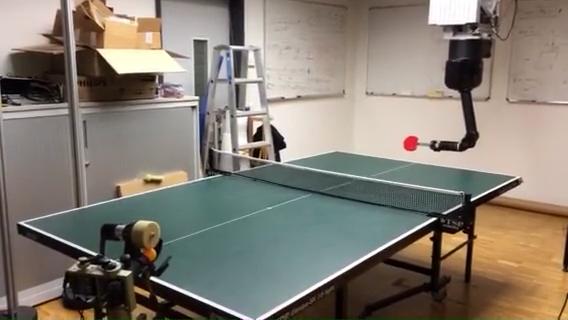
\includegraphics[scale=0.4]{robot1.png}			
\caption{Robotic table tennis setup with four cameras on the corners of the ceiling tracking the ball at 60 Hz. We filter the raw ball data provided from the cameras with an Extended Kalman Filter and predict the ball trajectory well in advance of the trajectory generation. A constrained nonlinear optimization problem is solved to find an optimal striking trajectory as well as an optimal striking time.}
\label{robot}
\end{figure}
% REPLACE PHOTO WITH ANOTHER ONE INCLUDING CAMERAS

Our contributions are two-fold. Firstly, we come up with an optimal control framework where the generation of striking trajectories are the result of an optimization problem. As opposed to previous works, we do not use any inverse kinematics or any fixed plane when computing joint trajectories. Secondly, we do not rely on the simplistic racket-ball reflection model when computing desired racket velocities and orientations. Instead, we train a probabilistic model based on human ball-racket demonstrations and use it to calculate cautious strategies for returning the ball.

In the rest of this paper, we describe the trajectory generation framework in detail. In Section~\ref{relatedWork} we introduce previous work on table tennis and other relevant trajectory generation frameworks. In Section~\ref{method} we formalize robot trajectory generation as a specific optimal control problem and incorporate probabilistic modeling within this framework. In Section~\ref{alg} we discuss a two-stage optimization approach for optimizing the previously introduced cost functional. In Section~\ref{results} we evaluate the performance of this approach and compare it with previous inverse kinematics (IK) approaches. Experiments in our robotic table tennis setup are given. In the final section~\ref{end} we discuss several promising extensions on this framework. %VHP-based

\begin{figure}[t!]
\centering
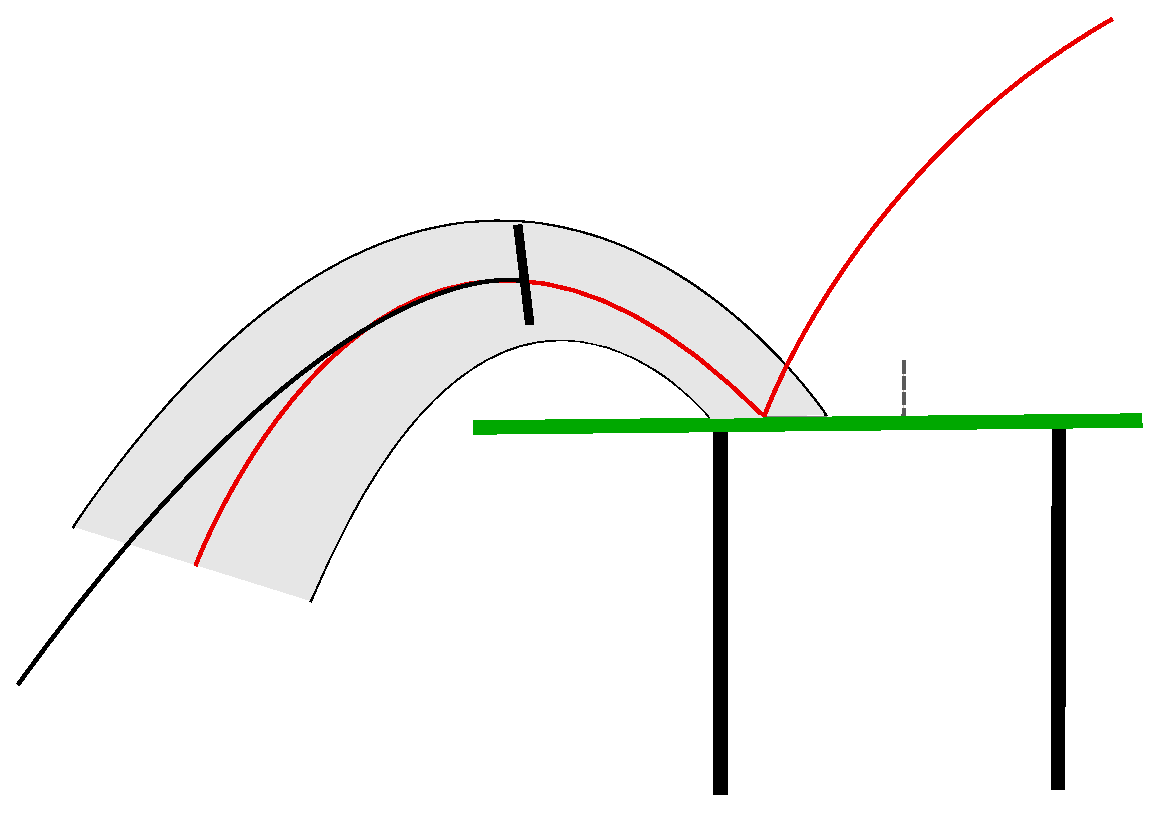
\includegraphics[scale=0.4]{drawing.eps}			
\caption{Illustrating the main idea behind this paper: fixing a virtual hitting plane (VHP) can make the generated trajectories unnecessarily restrictive and the resulting inverse kinematics may be infeasible. We instead consider the whole ball trajectory in our trajectory generation framework and optimize for the hitting time as well as the hitting point. Racket trajectory and the mean of the ball trajectory are shown in black and red, respectively. VHP is shown as a dotted gray line, the workspace of the robot is shown as an ellipsoidal light blue region.}
\label{mainIdea}
\end{figure}
%\section{TRAJECTORY GENERATION}\label{method}

In table tennis, one needs to specify when, where and how to intercept the incoming ball trajectory $\ball(t)$. So far, most of the algorithms for robotic table tennis \cite{Matsushima05}, \cite{Muelling13} calculate the intersection point of an estimated ball trajectory $\ballEst(t)$ with a virtual hitting plane $z = z_{\mathrm{VHP}}$ to determine the space and time coordinates of the hitting point. It is possible to eliminate this plane altogether and include the striking time as another parameter to be determined in an optimization problem.

\subsection{Optimal Control for Trajectory Generation}

When generating striking trajectories for the robot, trajectories with minimal acceleration or jerk can be preferred for safety and efficiency reasons. We therefore consider the following \emph{free-time} optimal control problem~\cite{Liberzon11}
%
\begin{align}
&\min_{\ddot{\joint},T} \int\limits_{0}^{T}\ddot{\joint}(t)^{\mathrm{T}}\vec{R}\ddot{\joint}(t), \label{costFnc1} \\
\textrm{s.t. \ } & \kin(\joint(T)) = [\normal_{\mathrm{des}}(t),\ballEst(t)], \label{transCond1}\\
&\jac(\joint(T))\dot{\joint}(T) = \racketVel_{\mathrm{des}}(t), \label{transCond2} \\
&\joint(0) = \joint_{0}, \label{initCond1} \\
&\dot{\joint}(0) = \dot{\joint}_{0}, \label{initCond2}
\end{align}
%
\noindent where the final time $T$ of the racket trajectory is an additional variable to be optimized along with the joint accelerations $\ddot{\joint}(t) \in \mathbb{R}^{n}$. The direct kinematics function $\kin(\cdot)  \in \mathbb{R}^{3 \times 2}$ is the relevant submatrix of the homogeneous transformation $\vec{T}(\cdot) \in \mathbb{R}^{4 \times 4}$ giving the desired racket normal and racket center position at striking time. The sub-Jacobian $\jac(\joint(T)) \in \mathbb{R}^{3 \times n}$ gives the condition for the desired Cartesian racket velocities. $\vec{R} \succeq 0 \in \mathbb{R}^{n \times n}$ is a positive definite weighting matrix for the accelerations. Initial conditions for the robot are the joint positions $\joint_0$ and joint velocities $\dot{\joint}_0$.

Solution of \eqref{costFnc1} using Pontryagin's maximum principle is well known in the optimal control literature: the solution $\joint(t)$ is a third degree polynomial for each degree of freedom, with the \emph{transversality conditions} \eqref{transCond1} - \eqref{transCond2} imposing another condition on the Hamiltonian to satisfy at striking time~\cite{Schaettler12}. See Figure~\ref{mainIdea} for an illustration. % which figure 

In the above case with only boundary equality constraints, the striking time $T$ and the joint position and velocity values at striking time $\joint_f$ and $\dot{\joint}_f$ fully parametrize the polynomial and can be determined by solving a $2n+1$ dimensional equation~\footnote{For example using $\mathtt{fsolve}$ in MATLAB.}. Inspired by the simplicity of this solution, we extend the same parametrization to the constrained optimization, with joint position, velocity and acceleration limits imposed throughout the whole trajectory.

\begin{figure}[t!]
\centering
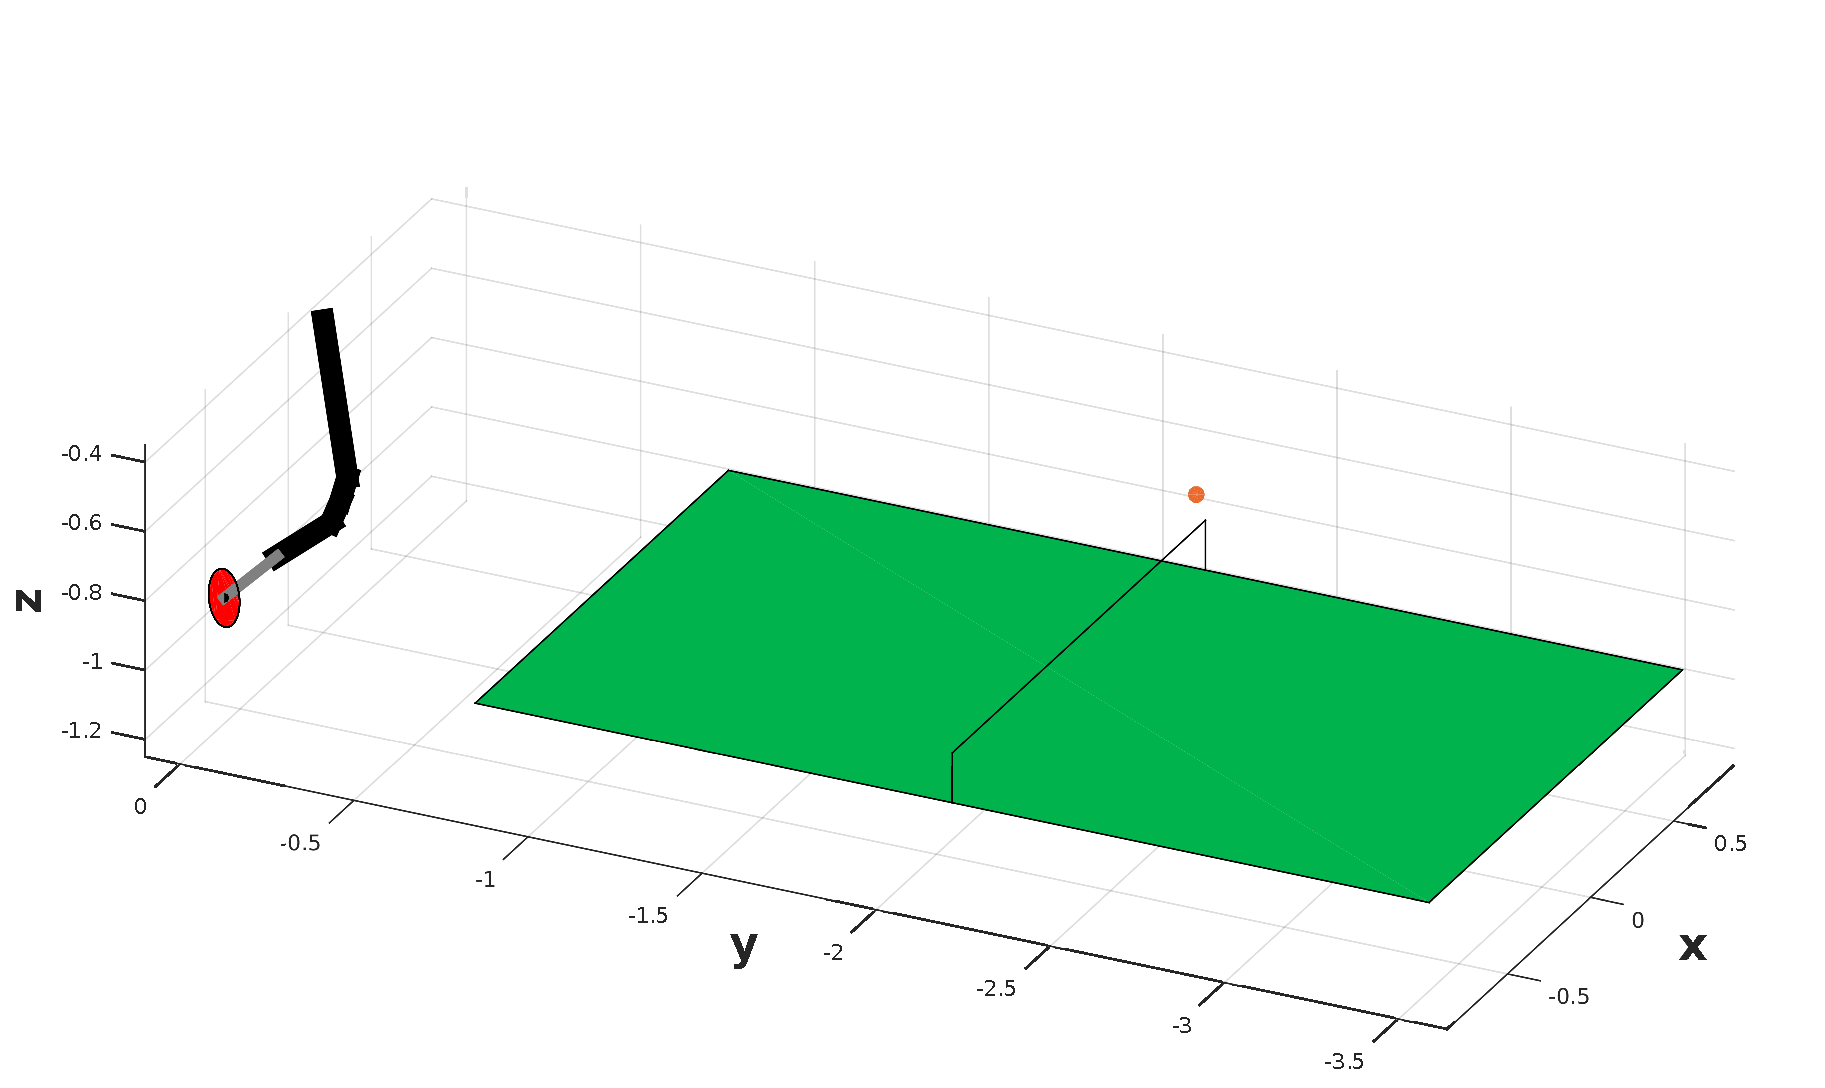
\includegraphics[scale=0.25]{tableTennis3D.eps}			
\caption{A schema for a three dimensional table tennis model. Ball is shown as an orange blob and the racket, in resting state, is shown in red. We predict the path of the ball using models that we train from actual data: the ballistic flight model, the rebound model and the racket-ball landing model respectively. The trajectory generation framework takes as input a desired racket trajectory calculated using these models.}
\label{models}
\end{figure}

\subsection{Predicting with Probabilistic Modeling}\label{sectionPredict}
 
In this framework, we require three models to determine the equality constraints~\eqref{transCond1} - \eqref{transCond2} for the trajectory generation process. We first need to predict the future ball trajectory $\ballEst(t)$ from noisy ball observations.  The ballistic \emph{flight model} is a nonlinear model $\ddot{\ball} = \ballDynamics(\dot{\ball})$ that describes the dynamics of the ball $\ball = (b_x,b_y,b_z)^{\mathrm{T}}$. It involves air drag $\drag$ and gravity $\gravity$
%
\begin{align}
\begin{bmatrix}
   \ddot{b_x} \\
   \ddot{b_y} \\
   \ddot{b_z}   
 \end{bmatrix} &= 
 \begin{bmatrix}
 -\drag \ballVel \dot{b}_x  \\
 -\drag \ballVel \dot{b}_y  \\
 \ \gravity - \drag \ballVel \dot{b}_z 
 \end{bmatrix},
\label{flightModel}
\end{align}
%
\noindent where $\ballVel = \|\dot{\ball}\|_2$ is the velocity of the ball. We use a linear model for the \emph{rebound model}
%
\begin{align}
\dot{\ball}_{\mathrm{out}} = \bounce\dot{\ball}_{\mathrm{in}}.
\label{reboundModel}
\end{align}

\noindent The rebound model \eqref{reboundModel} is a discrete event which reflects the ball when the ball is touching the table. Matrix $\bounce$ in \eqref{reboundModel} is a diagonal matrix with entries $\vec{\epsilon} = [\epsilon_{x}, \epsilon_{y}, -\epsilon_{z}]^{\mathrm{T}}$. The coefficient of restitution $\epsilon_{z} \in (0,1)$ accounts for the reflection of velocity in the vertical direction $z$ and $\epsilon_{x}, \epsilon_{y} \in (0,1)$ are the coefficients of friction along the planar $x,y$ directions. See Figure~\ref{models} for a table tennis schema. 

The accuracy of the rebound model~\eqref{reboundModel} clearly depends on that of the flight model~\eqref{flightModel}, so we first train the parameters of the flight model using nonlinear least squares. Secondly, we use the trained flight model to smoothen the ball path before rebound and after rebound. Using an Extended Kalman Smoother, we can calculate the ball velocities before and after rebound and then use linear least squares to estimate the rebound parameters. A more comprehensive approach would be to train the two models together with a smoothing Expectation-Maximization (EM) algorithm, at no apparent advantage. % cite needed
Effects of ball angular velocity, or in other words spin, are not accounted for in these models.

During test time we use the same trained Extended Kalman Filter (EKF) to perform prediction on the filtered ball state. Any other regression method to estimate initial ball position and velocity can also be used. Using an EKF for our nonlinear model \eqref{flightModel} generates at each time instant $t$ a probability distribution $p_t(\ball,\dot{\ball}|t)$ of incoming ball states parameterized by time, 
%
\begin{align}
\ball(t) &\sim \mathcal{N}(\vec{\mu}_{\textrm{in}}(t),\vec{\Sigma}_{\textrm{in}}(t)). 
\label{ballProcess}
\end{align}


%\section{Experiments}\label{experiments}

% is this necessary?
%\subsection{Experimental Setup}

In this section, we demonstrate the effectiveness of the algorithm presented in Section~\ref{algorithm} in the context of movement primitive learning for optimal striking motions. We consider two hitting tasks: putting in golf and ball-hitting in table tennis. In the first task the trajectory and the extracted movement primitives are assigned in operational, i.e. Cartesian space, whereas for the second task we generate these primitives in joint space, one for each joint of the robot. A low-gain feedback law is calculated in both cases using LQR with the linearized dynamics \eqref{discreteLTV} which transfers the weight updates of the DMPs to motor commands. The robustness that comes with the LQR feedback law and the DMP framework is an asset that strengthens the industrial applicability of our approach outside of the tested platforms.

We assume that the reference trajectories are \emph{feasible}, i.e. that it is possible to follow them arbitrarily well. If this assumption does not hold, then one can enforce feasibility by redesigning the basis functions $\basis(t)$ of the DMPs so as to filter out the nonsmooth parts of the trajectory adequately.

\subsection{Verification and Comparisons in Simulated Putting}

%Putting is a simple and natural domain for testing ILC algorithms because it allows a robot to apply ILC to actuate few degrees of freedom (typically the end joint) while having the dynamical effects from the other links act as disturbances. This kind of learning in underactuated dynamical systems can act as a scalable interface to more complex hitting tasks in the full-joint space of robots with high DoFs. Here we provide only a simple example to illustrate such \emph{scalable} learning.
%By learning the causal map of the disturbances acting on the robot (i.e. a graphical model) one can iteratively construct increasingly sophisticated controllers that are cognizant of the causal relationships between the joints and the disturbances. 

Putting is a simple and natural domain for testing ILC algorithms, in particular we consider it as a scalable interface to more complex hitting tasks with high DoF robots. We illustrate in Figure~\ref{putting1} a simplified simulation of a two-link planar arm with two revolute joints hitting a golf ball on the ground. We can imagine that a golf stick is attached to the end-effector at the second joint. We assume that we have available a circular reference trajectory that intercepts the ball with a desired velocity of $1.8$ m/s. This lets us account for the masses of the arm and the ball as well as a simulated kinetic friction of $\mu = 0.6$ between the golf ball and the ground. Good putting trajectories can be shown easily by expert humans or recorded via kinesthetic teach-in. 

In order to simulate learning with ILC, we assume that there is a model mismatch due to the motor inertia of both joints. We give the motor inertia a Gaussian distributed disturbance with zero mean and a variance of $0.05$, while the actual values of the motor inertia are $0.15$ and $0.12$ respectively. With these random disturbances we can construct error bars for $\alg$ and also test for the robustness of the proposed method.

\begin{figure}[ht]
\centering
\subfloat[Initial attempt]{%
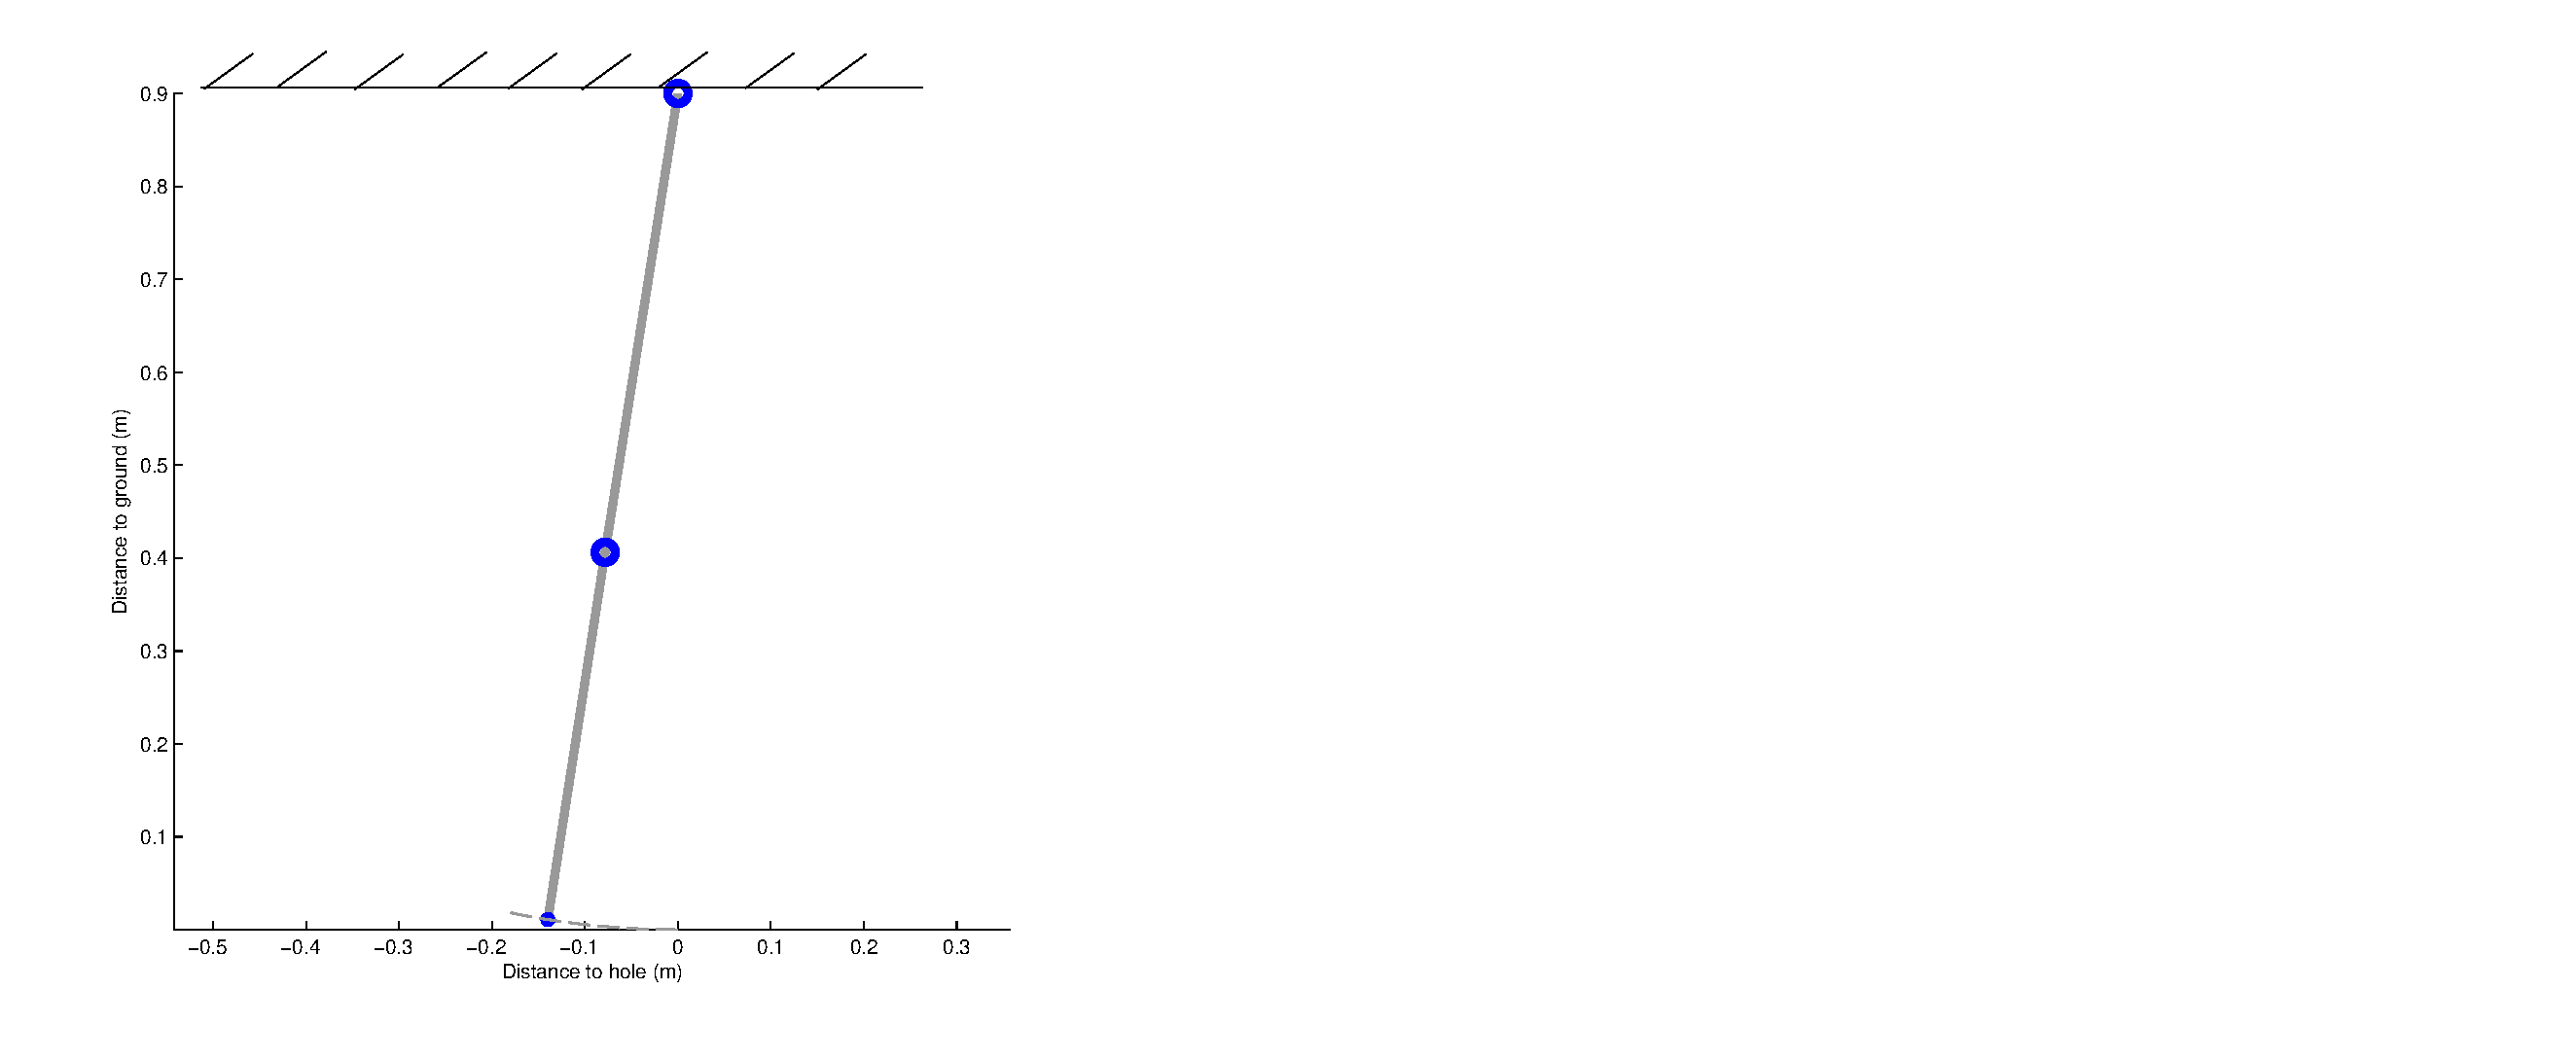
\includegraphics[width=0.5\linewidth]{putting0.eps}
\label{fig:subfig1}}
\subfloat[Final trajectory]{%
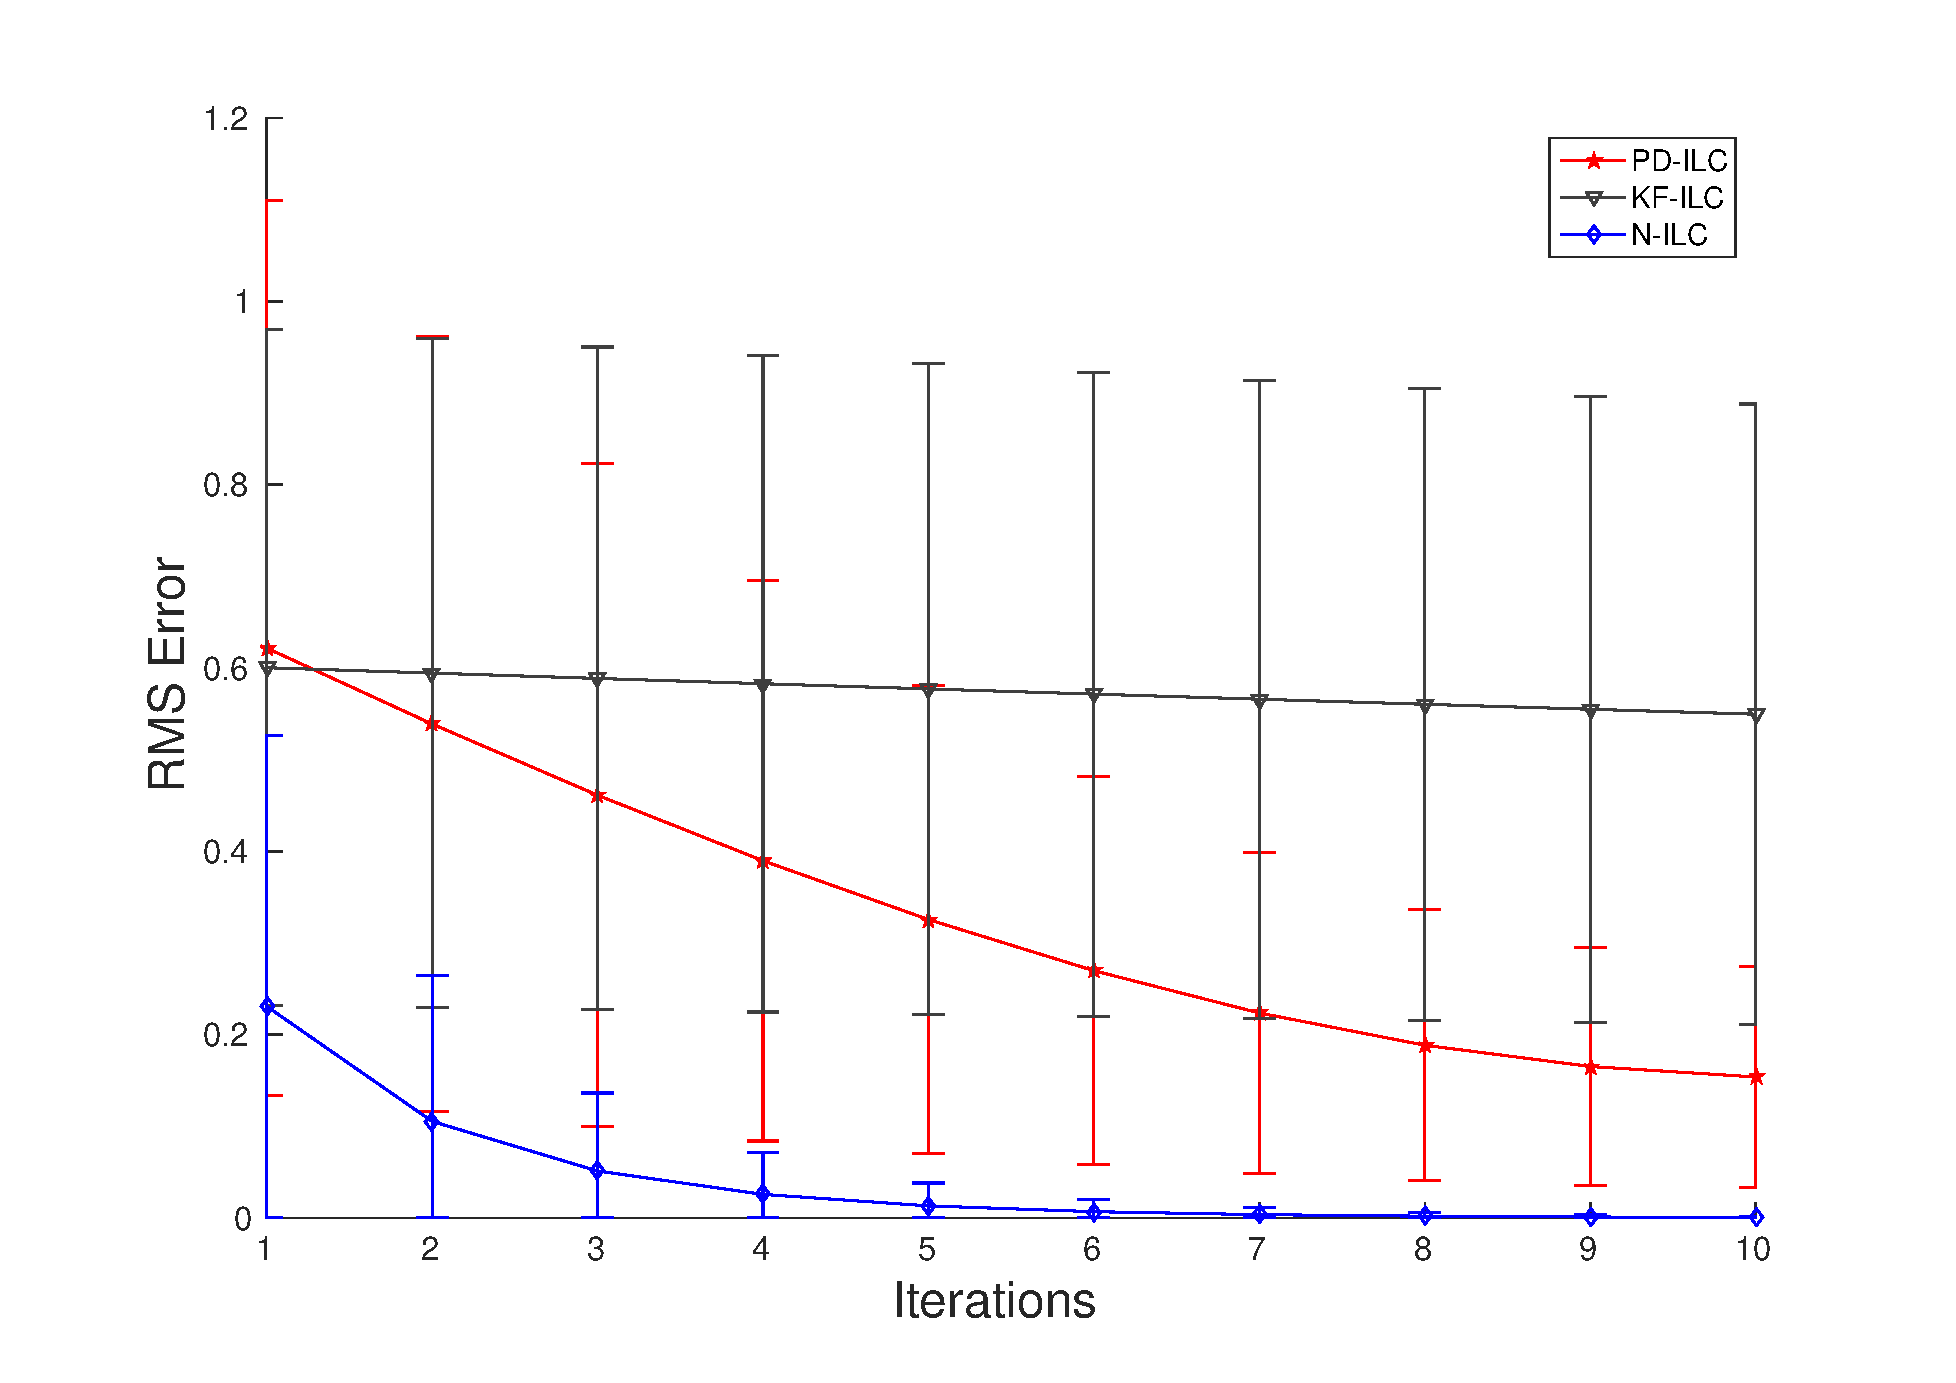
\includegraphics[width=0.5\linewidth]{putting1.eps}
\label{fig:subfig2}}
\caption{Robot arm must follow the assigned reference trajectory precisely in order to hit the ball with a desired velocity at the desired time. The reference trajectory is shown as a blue dashed curve. We can see in Fig.~\ref{fig:subfig1} that the initial attempt falls short of the reference trajectory. ILC then modifies the weights of the DMP to compensate for the modeling errors. In Fig.~\ref{fig:subfig2} the reference trajectory is executed perfectly. The ball will then approach the hole, shown as a thick blue line at a distance of 0.5 meters, with approximately zero velocity.} 
\label{putting1} 
\end{figure}

The iterations of \emph{wILC} are shown in Figure~\ref{wILCTrajectoryPutting}. Learning takes place in the joint space of the robot, since the matrix $\vec{F}_{w}$ is constructed using the nominal dynamics model \eqref{dynamics} in joint space. The full dynamics $\dynamics(\joint,\dot{\joint},\sysInput)$ involves the nonlinear effects from both links. We can see how initially the inertial disturbances of the motors prevent the end-effector from following the trajectory precisely. The following iterations show how ILC compensates for such an effect and in the last iteration the ball is given the desired velocity to reach the hole. We compare the approach with \emph{REPS} and \emph{PI$^{2}$} in Figure~\ref{wILCTrajectoryPutting} by plotting the RMS-error of the iterations with each algorithm. The error bars indicate one standard deviation within $10$ trials with different inertial mismatches. Notice that these stochastic approaches take much longer to converge.

% Compare alternative methods, gradient descent, etc.
% table shows that $R = 0$, $Q = I$ appears to be optimal in this case.

\begin{figure}
\center
%\includegraphics[scale=0.50]{comparison.eps}
\newlength\figureheight 
\newlength\figurewidth 
\setlength\figureheight{6cm}  
\setlength\figurewidth{6cm} 
\scalebox{1.0}{% This file was created by matlab2tikz.
% Minimal pgfplots version: 1.9
%
%The latest updates can be retrieved from
%  http://www.mathworks.com/matlabcentral/fileexchange/22022-matlab2tikz
%where you can also make suggestions and rate matlab2tikz.
%
\begin{tikzpicture}

\begin{axis}[%
width=0.95092\figurewidth,
height=\figureheight,
at={(0\figurewidth,0\figureheight)},
scale only axis,
separate axis lines,
every outer x axis line/.append style={black},
every x tick label/.append style={font=\color{black}},
xmin=0,
xmax=12,
xlabel={Iterations},
every outer y axis line/.append style={black},
every y tick label/.append style={font=\color{black}},
ymin=-0.05,
ymax=0.4,
ylabel={RMS Error},
title={Learning Performance in Putting},
legend style={legend cell align=left,align=left,fill=white}
]
\addplot [color=blue,solid]
 plot [error bars/.cd, y dir = both, y explicit]
 table[row sep=crcr, y error plus index=2, y error minus index=3]{%
1	0.233032343134884	0.118115271422138	0.118115271422138\\
2	0.0924719913705091	0.0562589335711811	0.0562589335711811\\
3	0.0384258808828579	0.0276274441478736	0.0276274441478736\\
4	0.0165387503761337	0.0138614543017086	0.0138614543017086\\
5	0.00733384353006482	0.00703352539176592	0.00703352539176592\\
6	0.00333781167932676	0.00358523371207059	0.00358523371207059\\
7	0.00155369907429323	0.0018294817119812	0.0018294817119812\\
8	0.000737146368162867	0.000933121803618784	0.000933121803618784\\
9	0.000355312489801426	0.000475460765776891	0.000475460765776891\\
10	0.000173512604061655	0.000241998267982427	0.000241998267982427\\
};
\addlegendentry{wILC};

\end{axis}
\end{tikzpicture}%}
\caption{Convergence of $\alg$ to the reference putting trajectory. Convergence is quadratic for the simulated scenario where we have unknown inertial disturbances acting on the motors. Note the slow and unstable performance of the other stochastic RL algorithms.}
\label{wILCTrajectoryPutting}
\end{figure}

\subsection{Application in Table Tennis}

% hitting is not at the end of the trajectory

As a second and more complex task, we consider table tennis where we are interested in generating and executing accurate ball-hitting motions. For the robotic table tennis task we are using a seven degree of freedom (DoF) torque-controlled Barrett WAM arm capable of high speeds up to X rad/sec. A standard size racket (16 cm diameter) is mounted on the end-effector of the arm as can be seen in Figure~\ref{robot}. A vision system consisting of four cameras hanging from the ceiling around each corner of the table is used for tracking the ball \cite{Lampert12}. The orange ball is tracked  visually with a sampling rate of 60 Hz and filtered with an extended Kalman filter that accounts for some of the bouncing behavior of the ball and air drag effects. The table and the tennis balls are in accordance with the International Table Tennis Federation (ITTF) rules.

A ball launcher (see Figure~\ref{ballgun}) is available to throw balls accurately to a fixed position in Cartesian space to the forehand of the robot. The incoming ball arrives with low-variability in desired positions and higher-variability in ball velocities. The whole area to be covered amounts to about 1 m$^2$ circular region in front of the initial forehand gesture of the robot. This allows us to avoid the singularities of the robot. Any ball that appears outside of this circular \emph{feasible} region will not be hit.

When the visual system provides a trajectory of the robot that coincides with the feasible region in Cartesian space, the system has to come up with a trajectory that specifies how, where and when to intersect the incoming ball trajectory. Desired Cartesian position, velocity and orientation of the racket translates in joint space to the specification of 14 parameters: 7 joint angles and 7 joint velocities of the robot arm. Along with the desired hitting time (or the time until impact), these 15 parameters are used to train 7 joint space DMPs that corresponds to the desired reference trajectory in Cartesian space. These movement primitives are synchronized with the same phase \eqref{phase}.

% maybe work on this kinesthetic teach-in paragraph more
In order to generate feasible reference trajectories that account for the variation in incoming ball position and velocity, we used kinesthetic teach-in on the robot to generate successful hitting motions, i.e. those that can hit the ball to the opponent's court. Using the successful examples we trained a probabilistic model $p(\weights|\state_b)$ given ball positions $\state_b$ using weighted regression. Weighting can be put in various ways and we opted for a weighting which put a higher reward on the fast strikes that landed on the edges. The generated DMPs of the model are guaranteed to be safe because these movements lie within the convex combination of demonstrations. 
% Katharina - Hence, the system will not encounter joint limits or hit the table.

% scale dmps if provided with better estimation data of ball position and velocity. dmps as opposed to control inputs or even trajectories can be easily extended to allow for this. 

% From Katharina's paper:
%the position, velocity and orientation of the racket can be computed analytically based on the state of the system and the target on the opponents court.
%These task space parameters can also be converted into joint space parameters using inverse kinematics

\begin{figure}
\center
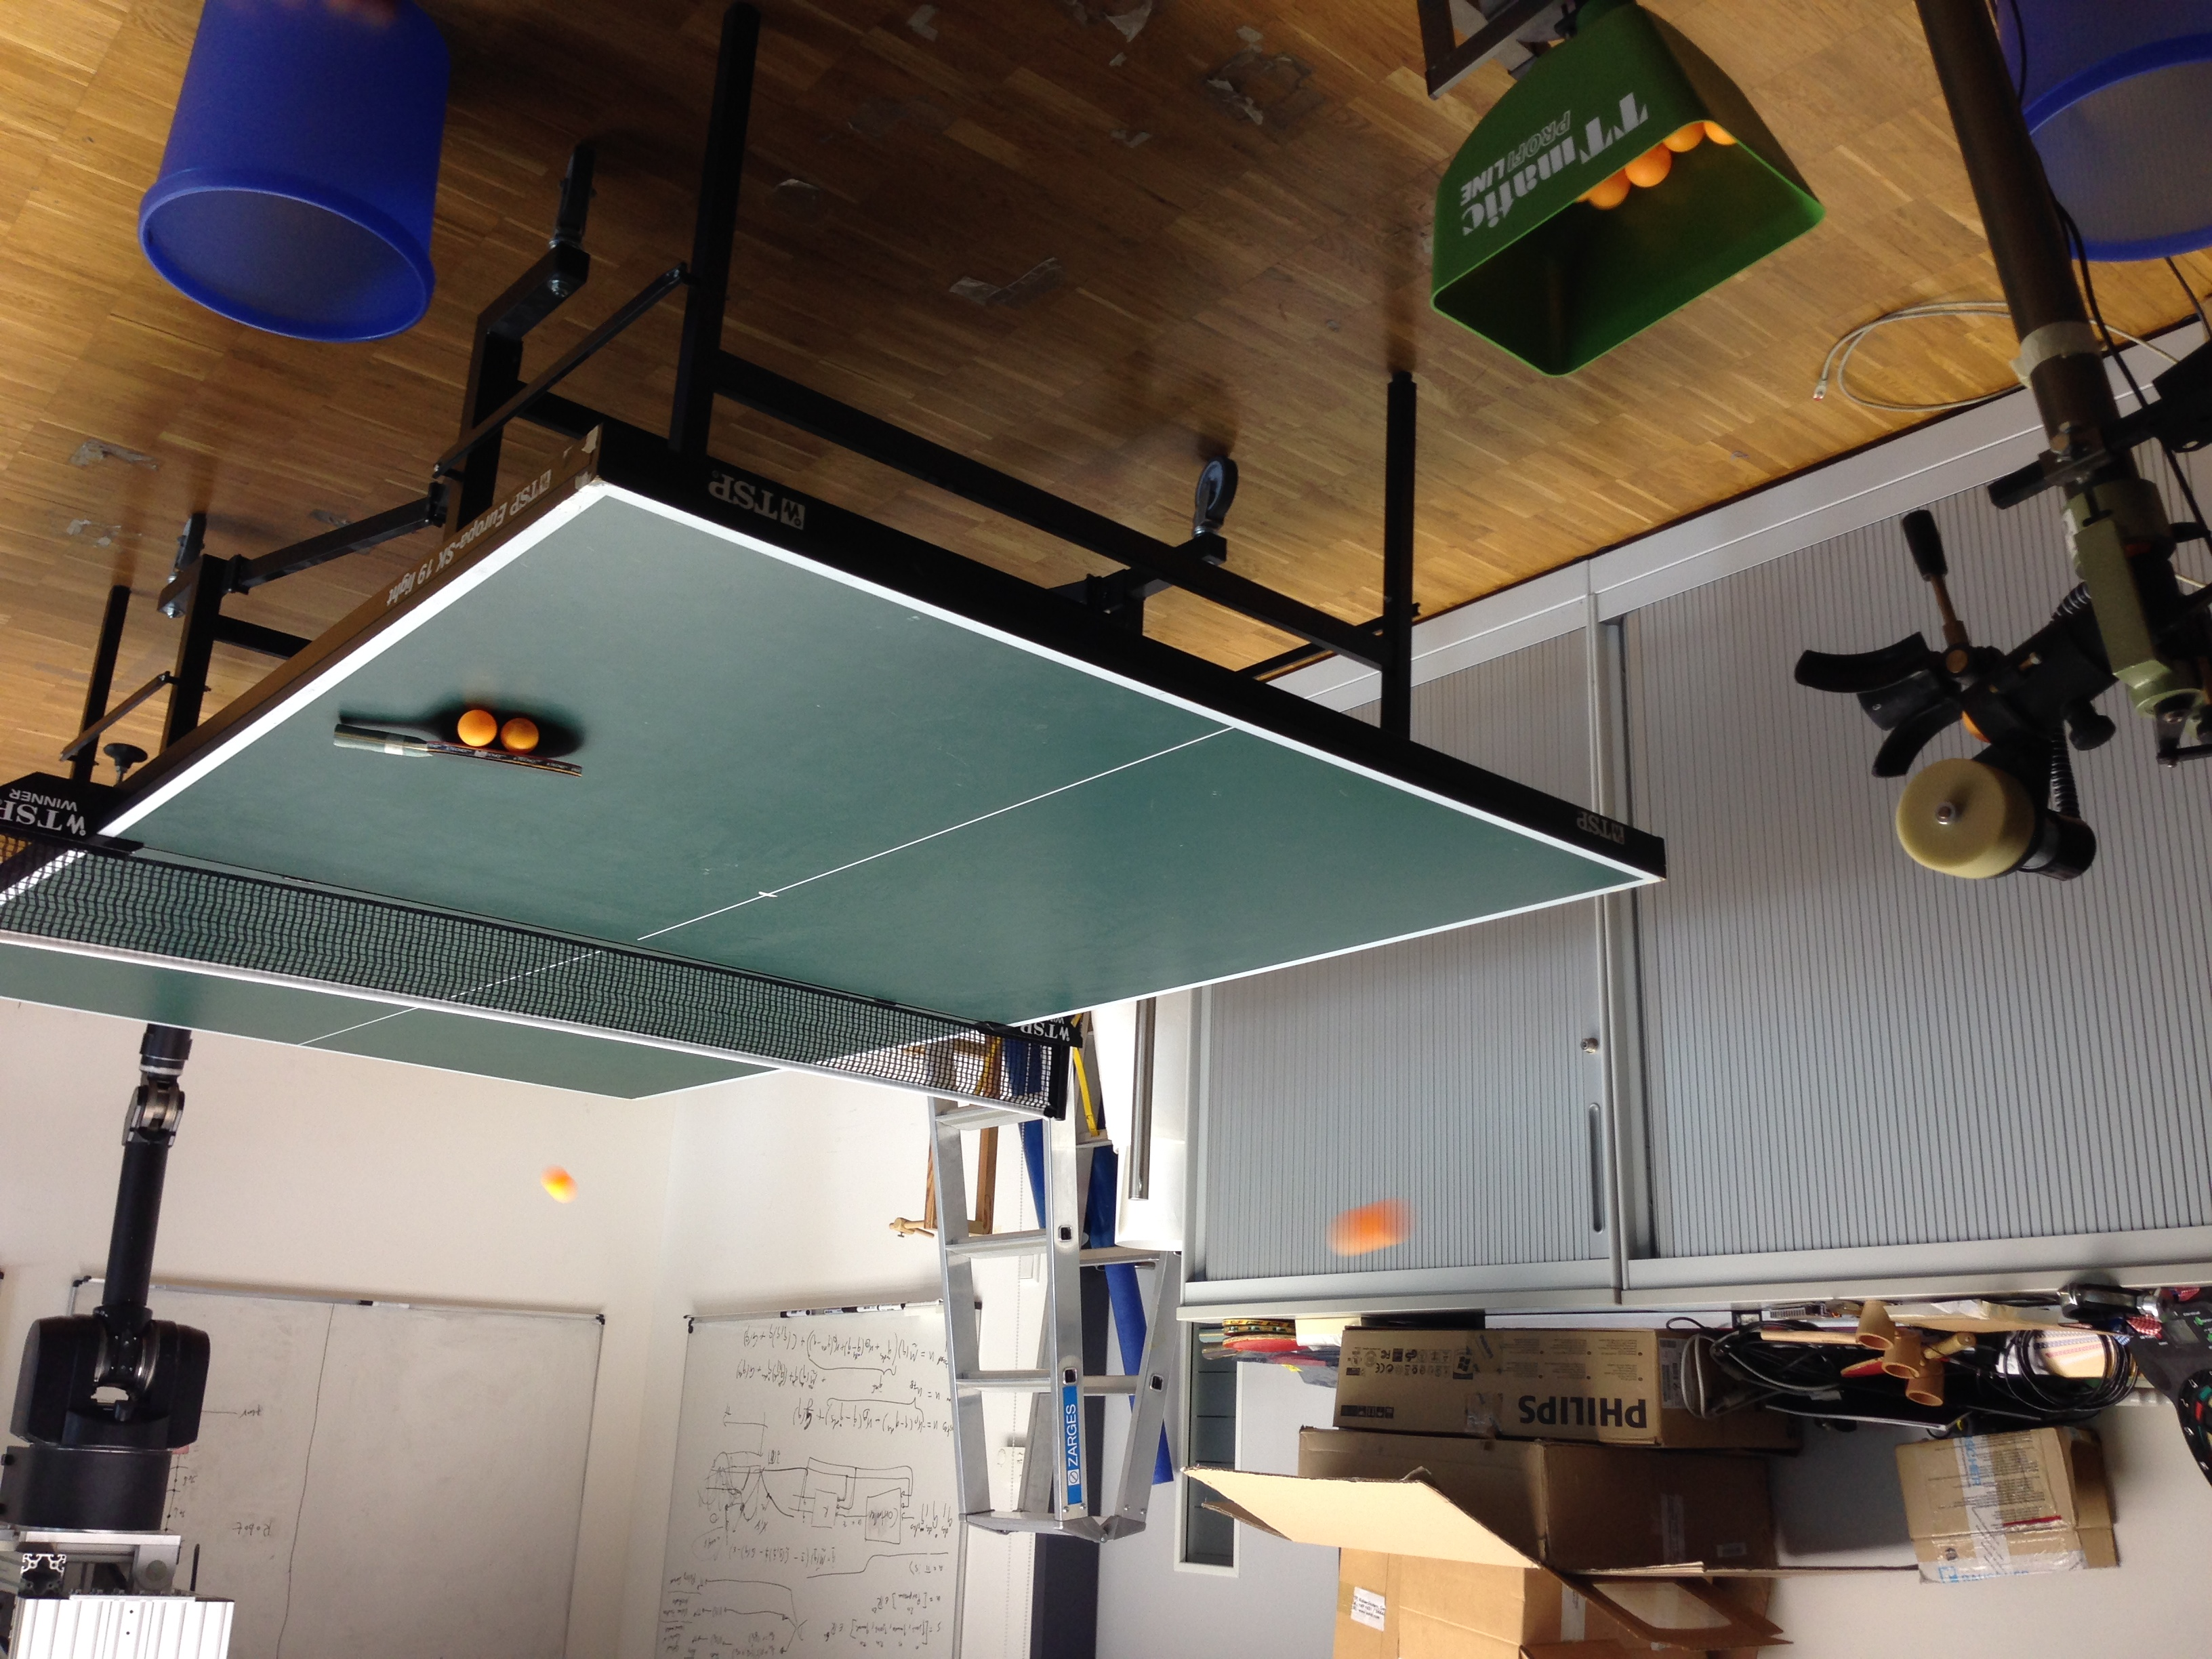
\includegraphics[scale=0.05, angle= 180]{ballgun.jpg}			
\caption{Robotic table tennis setup with the ball-launcher throwing balls to the robot}
\label{ballgun}
\end{figure}

The attached video shows the improvement achieved after using our algorithm $\alg$. In order to apply our method to a given reference trajectory, we use the mode of the empirical distribution $p(\weights,\state_b) = p(\weights|\state_b)p(\state_b)$ as the weights of our initial movement primitive. The convergence of the trajectories over the iteration domain are shown in Cartesian space in Figure~\ref{wILCTrajectoryTTCartesian}. Hard-to-model dynamical effects such as friction and stiction forces can be learned easily with our approach.

Comparisons to episodic-RL algorithms \emph{REPS} and \emph{PI$^{2}$} in Figure~\ref{ttComparison} illustrate the benefits of our approach, especially the faster convergence and increased accuracy of the proposed method. Some examples of the generated trajectories for the joints 5, 6 and 7 are given in Figure~\ref{wILCTrajectoryTT}. 

\begin{figure}
\center
%\includegraphics[scale=0.50]{comparison.eps}
\scalebox{1.0}{% This file was created by matlab2tikz v0.4.4 running on MATLAB 8.0.
% Copyright (c) 2008--2013, Nico Schlmer <nico.schloemer@gmail.com>
% All rights reserved.
% 
% The latest updates can be retrieved from
%   http://www.mathworks.com/matlabcentral/fileexchange/22022-matlab2tikz
% where you can also make suggestions and rate matlab2tikz.
% 
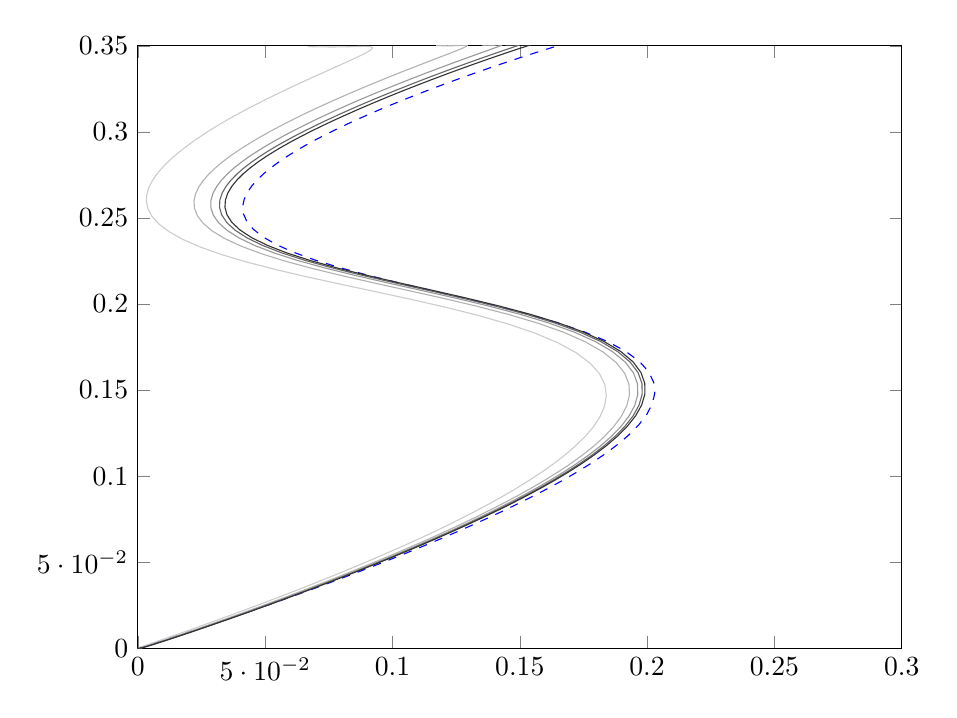
\begin{tikzpicture}

\begin{axis}[%
width=0.8\columnwidth,
height=0.630967741935484\columnwidth,
scale only axis,
xmin=0,
xmax=0.3,
ymin=0,
ymax=0.35
]
\addplot [
color=blue,
dashed,
forget plot
]
table[row sep=crcr]{
-1.22568529189217e-17 1.70219232680293e-47\\
-1.22078040529282e-17 2.17466204815869e-20\\
1.24930069097586e-15 5.59329658828069e-16\\
4.31962537102899e-13 1.9152423618868e-13\\
2.51770978879146e-11 1.11631432791867e-11\\
5.55015544523879e-10 2.46106431437956e-10\\
6.60280135771012e-09 2.9283319802688e-09\\
5.12320770129383e-08 2.27281407753508e-08\\
2.90255123674167e-07 1.28827401032052e-07\\
1.29124388293531e-06 5.73511237251698e-07\\
4.73949589296885e-06 2.10713748978966e-06\\
1.48681255318932e-05 6.6189380207418e-06\\
4.09129882041033e-05 1.82444393148059e-05\\
0.000100718153544017 4.50090857862532e-05\\
0.000225245856791989 0.000100919801590805\\
0.000463240655356511 0.000208196459707293\\
0.000884823147305501 0.000399120180670242\\
0.00158255610123486 0.000716854697447387\\
0.00266870907570527 0.00121464755420377\\
0.0042680934828865 0.00195306659807664\\
0.00650682428145541 0.00299533100932766\\
0.00949841893898853 0.00440125030957139\\
0.0133294488642299 0.00622065804358311\\
0.0180472586508033 0.00848740810159894\\
0.0236519674180277 0.0112149390444555\\
0.0300941529569334 0.0143941271208937\\
0.0372785249971626 0.0179937242124732\\
0.0450728081170337 0.0219632243456565\\
0.0533202318837492 0.0262376267222215\\
0.0618536166580361 0.0307433345872289\\
0.0705090712117028 0.0354043703208843\\
0.0791376965311413 0.0401481768418987\\
0.0876142690996799 0.0449104641836341\\
0.0958424961170963 0.0496387890730672\\
0.10375696557487 0.0542947727843779\\
0.111322280599518 0.0588550337458356\\
0.118530050316482 0.06331102120878\\
0.125394431996405 0.0676679861084513\\
0.131946828905364 0.0719433270169786\\
0.138230198729659 0.0761645191587581\\
0.144293265660084 0.0803667887860157\\
0.150184789161511 0.084590646654827\\
0.155947944238694 0.0888793518508938\\
0.161614820549927 0.0932763463165637\\
0.167201052648133 0.0978226842719481\\
0.172700648861156 0.102554481146252\\
0.178081188148765 0.107500424919056\\
0.183279696817351 0.112679429291778\\
0.188199689821794 0.11809856122523\\
0.192710046988842 0.123751440482291\\
0.196646565585241 0.12961737738435\\
0.199817148084927 0.135661573700226\\
0.202011400876493 0.141836677658674\\
0.20301387722613 0.148085506344443\\
0.202619789967853 0.154344644220661\\
0.20065273345486 0.160548886433011\\
0.196983021746862 0.166636203811203\\
0.191544736744952 0.172552738672092\\
0.184349409899893 0.178257268594913\\
0.175494381526898 0.183724581129977\\
0.165164317442443 0.188947295992029\\
0.153625080784607 0.193935846625374\\
0.1412100661361 0.198716567169214\\
0.12830006671719 0.203328087323888\\
0.115298606077758 0.207816473182085\\
0.10260527646616 0.212229725482657\\
0.0905898807700316 0.216612327368361\\
0.079570030652499 0.221000508160764\\
0.0697943393352088 0.225418764413873\\
0.0614325578259062 0.229877979341309\\
0.0545730774278078 0.234375244026284\\
0.0492273137352959 0.238895250492305\\
0.0453397371877769 0.243412935431724\\
0.0428018209176867 0.247896930561529\\
0.0414679809317703 0.252313332254143\\
0.0411716730700138 0.25662933480681\\
0.0417402386729666 0.260816396765839\\
0.0430079265640447 0.264852853167071\\
0.0448258671359753 0.268725657669276\\
0.0470681659059565 0.272431034965027\\
0.0496347242551211 0.275974250701863\\
0.0524515935766653 0.279368747748684\\
0.0554695907154709 0.282634858417776\\
0.0586617700544091 0.285798252905515\\
0.0620201947143181 0.288888235420426\\
0.0655523003124128 0.291935958228636\\
0.0692770158504934 0.294972594140621\\
0.0732207080290693 0.298027491449363\\
0.0774129544020573 0.301126332090716\\
0.0818821323091202 0.304289323201106\\
0.086650838109129 0.307529473239184\\
0.0917312255322955 0.310851034404806\\
0.0971204675308709 0.314248229434997\\
0.102796687767279 0.317704416545961\\
0.108715848493778 0.321191871765943\\
0.114810181592199 0.324672370955634\\
0.120988762173356 0.328098721508834\\
0.127140705706413 0.3314173160038\\
0.133141194808927 0.33457165455712\\
0.138860120113893 0.33750661939838\\
0.14417260737948 0.340173109510588\\
0.148970203575231 0.342532494031226\\
0.15317114157554 0.344560265930261\\
0.156728025765686 0.346248311683806\\
0.159631560364095 0.347605376663323\\
0.16190957122079 0.348655584952959\\
0.163621436389131 0.349435214610502\\
0.164848937801264 0.349988255460754\\
0.165685237911466 0.350361500346063\\
0.166223974647865 0.350599977591089\\
0.166550272189824 0.350743403168433\\
0.166734851771187 0.350824053127807\\
0.166831595215191 0.350866113799758\\
0.166878121826248 0.350886259282569\\
0.166898406741448 0.350895013534916\\
0.166906302339804 0.350898412202254\\
0.16690899217171 0.35089956776726\\
0.166909773384699 0.350899902896113\\
0.166909959992641 0.350899982867216\\
0.166909994843181 0.350899997792469\\
0.166909999566499 0.350899999814467\\
0.166909999980335 0.350899999991584\\
0.166909999999663 0.350899999999856\\
0.166909999999999 0.3509\\
0.16691 0.3509\\
0.16691 0.3509\\
};
\addplot [
color=white!80!black,
solid,
forget plot
]
table[row sep=crcr]{
-1.22568529189217e-17 1.70219232680293e-47\\
3.25274463507264e-06 8.35905362814104e-08\\
1.23717401990733e-05 6.51809556987925e-07\\
2.60782198962572e-05 2.10499070948953e-06\\
4.3092311772854e-05 4.74258914527822e-06\\
6.21318876894655e-05 8.7637958130708e-06\\
8.19125001256813e-05 1.42692959778432e-05\\
0.000101156688969535 2.12681872858731e-05\\
0.000118643983994053 2.97049649157848e-05\\
0.000133386193364771 3.95467615229986e-05\\
0.00014510004883005 5.10128278393354e-05\\
0.0001552465101183 6.5075416432896e-05\\
0.000168952051477796 8.43854757627399e-05\\
0.000198041564834851 0.000114740042164133\\
0.00026513772561189 0.000167083224948609\\
0.000408333337430968 0.000259824989119074\\
0.000685436662127054 0.000421023858453292\\
0.00117641921404975 0.000689800526123193\\
0.0019826628090404 0.0011163219128708\\
0.00322202345439749 0.00175987161326193\\
0.00501956323556232 0.00268488373870233\\
0.00749484404363355 0.0039552731473001\\
0.0107476267088559 0.00562781764097272\\
0.0148443828740994 0.00774561614639042\\
0.0198080260882525 0.0103326877885853\\
0.0256126991972536 0.0133905843814564\\
0.0321844810802911 0.0168975212907577\\
0.0394077642119747 0.0208100876679215\\
0.0471360843591468 0.0250671836813051\\
0.0552055623017432 0.0295955336269499\\
0.0634489323010695 0.0343159814489065\\
0.0717083475272989 0.0391497861089964\\
0.0798456440508612 0.0440242623581138\\
0.0877493512990643 0.0488773077339653\\
0.0953383119334656 0.0536605715857425\\
0.102562219474309 0.0583412200179673\\
0.109399655339149 0.0629024072076402\\
0.115854312001125 0.0673426650555623\\
0.121950058891251 0.0716744673315447\\
0.127725389733361 0.075922219782685\\
0.133227633162548 0.0801198897574413\\
0.138507154146251 0.0843084353295575\\
0.143611650722376 0.0885331395891004\\
0.148580574700905 0.0928409108464387\\
0.15343968194199 0.0972775796199095\\
0.158195747221979 0.101885211071146\\
0.16283155730666 0.106699458175359\\
0.16730141867135 0.111747006834142\\
0.171527575073714 0.117043208571809\\
0.175398110794516 0.122590056608926\\
0.17876709519038 0.128374731727528\\
0.181457870007442 0.13436901784707\\
0.183270418807971 0.140529933609352\\
0.183992840168584 0.1468017196852\\
0.183415811647512 0.153118883204305\\
0.181349255134415 0.159410354303193\\
0.177640391773053 0.165604747985411\\
0.172191559796912 0.171636409453042\\
0.164975852452944 0.177451555876\\
0.156048491179281 0.183013478959773\\
0.145551999572995 0.188305754446059\\
0.133713873420574 0.193332875414501\\
0.120836446899598 0.198118387394409\\
0.107279687175711 0.202701044925459\\
0.0934385122850055 0.207129644586298\\
0.0797168904764897 0.211457183163945\\
0.0665013860742654 0.215734973676006\\
0.0541368781104964 0.22000733245879\\
0.0429068577808264 0.224307382025773\\
0.033020059316166 0.22865437252083\\
0.0246043139118881 0.233052722129095\\
0.0177075894370749 0.237492749893384\\
0.0123053407655547 0.241952864909341\\
0.00831266795198405 0.246402818708713\\
0.00559943353492465 0.250807543394727\\
0.00400643982833325 0.255131090794861\\
0.00336099531970944 0.259340261583538\\
0.00349094963575494 0.263407694601951\\
0.00423632700566043 0.267314287640521\\
0.00545739698604056 0.271050520324513\\
0.00703909360281847 0.274616713655985\\
0.00889256053514898 0.278022468888926\\
0.0109545952245223 0.281285525081238\\
0.0131856580959084 0.284430233952467\\
0.0155669691751959 0.28748580297281\\
0.018097061806758 0.290484411403001\\
0.0207880223567336 0.293459265457746\\
0.0236615294186096 0.296442631788672\\
0.0267447249692657 0.29946387492171\\
0.0300659091430229 0.30254752444948\\
0.0336500541993982 0.305711411122957\\
0.0375141841333209 0.308964936070606\\
0.0416627620032532 0.312307571339502\\
0.0460833573873633 0.315727727789735\\
0.0507430103470991 0.319202160247643\\
0.0555858324175085 0.322696098963651\\
0.0605324459864692 0.326164288076076\\
0.0654818150895609 0.32955306358398\\
0.0703158276701347 0.332803506928079\\
0.0749066424601935 0.335855565592948\\
0.0791263436331281 0.338652851337519\\
0.0828579300985524 0.341147637015078\\
0.086006219944052 0.343305417717783\\
0.0885070089368458 0.345108336437797\\
0.0903329042299405 0.34655685170897\\
0.0914947162488735 0.34766926934375\\
0.0920380775007132 0.348479140774549\\
0.0920358866418595 0.349030952794802\\
0.0915779982342309 0.349374872001687\\
0.0907600654711163 0.349561458970446\\
0.0896734678021941 0.349637195188974\\
0.0883978262579761 0.349641406227386\\
0.0869968669564486 0.349604803855963\\
0.0855175674063735 0.349549511893666\\
0.0839918507219313 0.349490176744121\\
0.0824397444046635 0.349435647523352\\
0.0808729297318141 0.349390745172857\\
0.0792978877849283 0.349357781483348\\
0.0777182414268251 0.349337669415243\\
0.076136245249234 0.349330621539781\\
0.0745535944675742 0.349336526488321\\
0.0729717944868774 0.349355120123051\\
0.0713922993651467 0.349386049440274\\
0.0698165526897378 0.34942889134331\\
0.068245996566624 0.349483156689842\\
0.0666820730088789 0.349548290832413\\
};
\addplot [
color=white!70!black,
solid,
forget plot
]
table[row sep=crcr]{
-1.22568529189217e-17 1.70219232680293e-47\\
6.93129473689265e-06 9.64767466645037e-08\\
2.7053728010589e-05 7.53393712416719e-07\\
5.90241087723482e-05 2.43942373846901e-06\\
0.000101498155661405 5.51343408114195e-06\\
0.000153129376081493 1.02251741061884e-05\\
0.000212569038951388 1.67171588199604e-05\\
0.000278475522813864 2.50317808145982e-05\\
0.000349564364216304 3.51385921991254e-05\\
0.000424783594102553 4.70220206280164e-05\\
0.000503786426983947 6.09116511278121e-05\\
0.000587970596547154 7.77844535591212e-05\\
0.000682399652245789 0.000100292595867371\\
0.000798835848869633 0.000134233849753492\\
0.000959839481982006 0.000190556312586955\\
0.00120344120098727 0.000287681051323386\\
0.00158738733147519 0.000453687794298591\\
0.00219158773190882 0.000727729550523115\\
0.00311736305544096 0.00116001496346112\\
0.00448250910290361 0.00180987440428384\\
0.00641202948157397 0.00274178773012311\\
0.00902543036526304 0.00401970807708507\\
0.0124224207575113 0.00570043852896392\\
0.0166694253808309 0.00782708640457289\\
0.0217893165013838 0.0104236601922089\\
0.0277562016851992 0.0134916813674616\\
0.0344961305342789 0.0170093156475479\\
0.0418934719326902 0.0209330844092612\\
0.0498017431838193 0.025201803884487\\
0.0580570510257657 0.0297421012468949\\
0.0664921193903008 0.0344747144410509\\
0.0749490943067283 0.0393207933494284\\
0.083289807743699 0.0442075475846333\\
0.0914027883802557 0.0490727809439252\\
0.0992068821701957 0.053868067178828\\
0.106651790765752 0.0585605198516327\\
0.113716109160424 0.0631332660419391\\
0.120403549051503 0.0675848357938546\\
0.12673800451864 0.0719277239249715\\
0.132757998825081 0.0761863763987518\\
0.138510894368985 0.0803948155499262\\
0.144047093460022 0.0845940647197951\\
0.149414334532967 0.0888294783218773\\
0.154652112482077 0.0931480382373108\\
0.159786228723888 0.0975956474153343\\
0.164823505971776 0.102214439249045\\
0.169746781305514 0.107040127859175\\
0.174510413938733 0.1120994503015\\
0.179036702853095 0.11740779612371\\
0.183213790070021 0.122967179842902\\
0.186895805137288 0.128764782568114\\
0.1899061521658 0.134772362639757\\
0.192044878582981 0.1409468819141\\
0.193100147022395 0.1472324882047\\
0.19286269715242 0.153563556499437\\
0.19114250810376 0.159868847403178\\
0.187786850523484 0.166076780850869\\
0.182698103454159 0.172121506524738\\
0.175849394842952 0.177949080546467\\
0.167295979727899 0.183522700154989\\
0.157180417585707 0.188825927304757\\
0.145730241246288 0.193863312442234\\
0.133247818825882 0.198658504269697\\
0.120093144190204 0.203250378202201\\
0.106661152660102 0.207687847535028\\
0.0933558199927957 0.212024008470429\\
0.0805637088347397 0.216310250212964\\
0.0686296882127832 0.220590940806223\\
0.0578372317943576 0.224899231308802\\
0.0483950494317936 0.229254379779297\\
0.0404309416589472 0.233660794691578\\
0.0339928399182604 0.238108770890859\\
0.029056157412647 0.242576681968768\\
0.0255359478476862 0.247034235902087\\
0.0233020233782072 0.25144631659818\\
0.022195132642067 0.255776926658629\\
0.0220425280052933 0.259992820280044\\
0.0226720014664253 0.264066596454024\\
0.0239235191055781 0.267979123522436\\
0.0256572927278969 0.271720864841182\\
0.0277581997534111 0.275292139685674\\
0.0301373289229437 0.278702562031931\\
0.0327314247052732 0.281969896717172\\
0.0355008966451315 0.285118531913417\\
0.0384269160159032 0.288177719212875\\
0.0415079695590667 0.29117968640564\\
0.0447560992523834 0.294157689412887\\
0.0481929416503832 0.297144042766935\\
0.0518455992455894 0.300168154376497\\
0.0557423354994946 0.303254590408189\\
0.0599080890900244 0.306421209410366\\
0.0643598537911934 0.309677429863546\\
0.0691020660270022 0.313022729303285\\
0.0741222724777841 0.31644551101468\\
0.0793874940891376 0.319922508214131\\
0.0848418269794431 0.3234189148495\\
0.0904058815988261 0.326889423920117\\
0.0959786131876827 0.330280306170263\\
0.101441903661408 0.333532565762175\\
0.106667908232484 0.336586064933916\\
0.111528710145165 0.339384328716674\\
0.115907310598752 0.341879550643571\\
0.119708534372898 0.344037164229383\\
0.12286818970643 0.345839278347961\\
0.125358902890373 0.347286351236394\\
0.127191509935881 0.348396722962202\\
0.128411673995255 0.349204008280944\\
0.129092327454437 0.349752776234616\\
0.129323359924559 0.350093282717987\\
0.129200459903221 0.350276173935389\\
0.128815042047515 0.350348005584898\\
0.128246762583773 0.350348161750893\\
0.127559383036323 0.350307395802087\\
0.126799916704839 0.350247857240857\\
0.126000322945996 0.350184204555702\\
0.1251806659329 0.350125288184074\\
0.124352663973483 0.350075922368641\\
0.123522835457299 0.350038406444803\\
0.122694840758248 0.350013636784894\\
0.12187097212178 0.350001806250653\\
0.12105296251271 0.350002781183144\\
0.120242355145558 0.350016272815784\\
0.119440641921753 0.350041901264811\\
0.11864930428768 0.350079214324527\\
0.117869822211852 0.350127691516173\\
0.117103675565859 0.350186744625179\\
};
\addplot [
color=lightgray!80!black,
solid,
forget plot
]
table[row sep=crcr]{
-1.22568529189217e-17 1.70219232680293e-47\\
8.24119022140355e-06 1.00732406791694e-07\\
3.22818627429921e-05 7.86940656335505e-07\\
7.07559323208588e-05 2.54986090125147e-06\\
0.000122296228331723 5.76797064381405e-06\\
0.00018553338427912 1.07077012838254e-05\\
0.000259095822954879 1.75253638232066e-05\\
0.000341619118787306 2.62743262033844e-05\\
0.000431796062051802 3.69323957213372e-05\\
0.000528552011866369 4.94896975186751e-05\\
0.000631517600857057 6.41792322979517e-05\\
0.000742068082289762 8.19795699039566e-05\\
0.000865244631480491 0.000105543401475197\\
0.00101278723256497 0.000140668999415314\\
0.00120723400539919 0.000198306249405875\\
0.00148659350872234 0.000296880649727077\\
0.00190859005869599 0.000464480052181126\\
0.002553111603022 0.000740269632660934\\
0.00352145704973565 0.00117447363800878\\
0.00493140077336401 0.00182643993469807\\
0.00690792553655244 0.00276066560601727\\
0.00957051760868816 0.00404111845209194\\
0.013018867428092 0.00572461167681009\\
0.0173193828571617 0.00785425676069301\\
0.0224949212787883 0.0104540595927566\\
0.0285195774988574 0.0135255320009586\\
0.035319390500034 0.017046823099313\\
0.0427787205908372 0.0209744310901322\\
0.0507510783541073 0.0252471431363759\\
0.0590725654150967 0.0297915525019845\\
0.0675759019452456 0.0345283599239281\\
0.0761032313718057 0.0393786768622851\\
0.0845163841555275 0.0442696758156739\\
0.0927038886619868 0.0491391274533087\\
0.100584591960087 0.0539385788040041\\
0.108108198522499 0.0586351248731017\\
0.115253308079248 0.0632118832043138\\
0.122023639052197 0.0676673832532119\\
0.128443094156398 0.0720141273595286\\
0.134550207016313 0.076276575782572\\
0.140392351886249 0.0804887703534101\\
0.146019944204992 0.0846917575060123\\
0.151480736630151 0.0889309168345366\\
0.156814239248724 0.0932532561315467\\
0.162046269569075 0.0977047037845897\\
0.167183667267311 0.102327417068251\\
0.172209287258199 0.107157131409542\\
0.177077507480326 0.112220601573851\\
0.181710646551086 0.117533230120374\\
0.18599686704668 0.123097038618307\\
0.189790319960976 0.128899207779441\\
0.192914431638598 0.134911486360631\\
0.195169272283309 0.141090815579626\\
0.196343027377081 0.147381309838045\\
0.196226458744299 0.153717296801278\\
0.194629565937674 0.160027476514049\\
0.191399637271586 0.166240199323007\\
0.18643906636242 0.172289545207232\\
0.179720993560132 0.178121512882846\\
0.171300685919523 0.183699265895567\\
0.16132071575316 0.189006361231044\\
0.15000862915004 0.194047369705262\\
0.137666806389296 0.198845976718071\\
0.124655250930212 0.203441100722334\\
0.11136890434015 0.207881696624692\\
0.0982117451440555 0.212220896144709\\
0.0855703354850615 0.216510115804387\\
0.0737895409198586 0.220793742315416\\
0.0631528289654475 0.225104937212302\\
0.0538689008840692 0.229462961720491\\
0.0460655463836004 0.233872221219448\\
0.0397906840306257 0.238323002294295\\
0.0350197122887116 0.242793666223433\\
0.0316676684619934 0.247253905761631\\
0.0296043468694794 0.251668587890903\\
0.0286704771406535 0.256001697867092\\
0.0286932917590319 0.260219973468202\\
0.0295005622973088 0.264295999581883\\
0.0309322342141809 0.268210634111924\\
0.0328484988224416 0.271954334638874\\
0.0351342134438643 0.275527419817031\\
0.0377004473008033 0.278939508125996\\
0.0404839260303129 0.282208373537663\\
0.0434450410789383 0.285358417140878\\
0.0465649463701479 0.288418906155873\\
0.0498421120540551 0.291422085547991\\
0.0532885643012866 0.294401228807807\\
0.0569259246939338 0.297388667359027\\
0.060781281661924 0.300413824369689\\
0.0648828856070467 0.303501278808989\\
0.0692556632508983 0.306668898869657\\
0.0739165976105503 0.309926108924857\\
0.0788701156320308 0.313272388148497\\
0.0841037558484537 0.316696136786902\\
0.0895845324026466 0.320174080001135\\
0.0952565359222051 0.323671398441293\\
0.101040372596916 0.327142766524831\\
0.106834994514794 0.330534431396352\\
0.112522281411398 0.333787369354094\\
0.117974387199522 0.336841411957749\\
0.123063394734693 0.339640053057411\\
0.127672305965782 0.342135457664629\\
0.131705947986898 0.344293037104961\\
0.135100133412516 0.346094887844805\\
0.137827495291969 0.3475414677501\\
0.139898878703717 0.348651128804713\\
0.141359957684072 0.349457508011248\\
0.142283676615549 0.350005203379756\\
0.142759937586791 0.350344502272953\\
0.142884441669828 0.350526081058766\\
0.142748616062309 0.350596521548441\\
0.14243212952282 0.350595228378737\\
0.141998756175451 0.350552969484934\\
0.141495522047665 0.350491903311688\\
0.140954399376044 0.350426692491499\\
0.140395465359062 0.350366187815311\\
0.13983045145243 0.350315201062375\\
0.139265889288576 0.350276027090483\\
0.138705452554353 0.350249556355617\\
0.138151446857674 0.350235974722749\\
0.137605618559151 0.350235140647284\\
0.13706952429002 0.350246756673952\\
0.136544669380156 0.350270433458172\\
0.136032548709625 0.350305708569233\\
0.135534655681571 0.350352050539719\\
0.135052483600492 0.350408859401613\\
};
\addplot [
color=gray!80!black,
solid,
forget plot
]
table[row sep=crcr]{
-1.22568529189217e-17 1.70219232680293e-47\\
8.92977877512262e-06 1.02875256139306e-07\\
3.50302073670603e-05 8.03832204998465e-07\\
7.6923181451443e-05 2.6054666526772e-06\\
0.000133229513849615 5.89612735388159e-06\\
0.000202567829414407 1.09506412435071e-05\\
0.000283554556587495 1.79322606298721e-05\\
0.000374813297083546 2.68998738572252e-05\\
0.000475024898264518 3.78354390567461e-05\\
0.00058310281472824 5.07319460217592e-05\\
0.000698665821066556 6.58241162764799e-05\\
0.000823077365168913 8.40913381849907e-05\\
0.000961366872516901 0.000108186603085048\\
0.00112526263206191 0.000143908514171362\\
0.0013372911192877 0.000202208001417812\\
0.00163544929455634 0.000301513027909894\\
0.00207744991934694 0.000469915878014372\\
0.00274316943818554 0.00074658831036123\\
0.00373389534015586 0.0011817629856139\\
0.00516739074226722 0.00183479720468099\\
0.00716862744585325 0.00277019737138397\\
0.00985708124108685 0.00405193928677507\\
0.0133324327779902 0.00573684179051188\\
0.017661081015106 0.00786801888227079\\
0.0228658754619511 0.0104694754201866\\
0.0289209041629876 0.0135427184867887\\
0.0357522004656874 0.0170658887717894\\
0.0432441201229809 0.0209954725658302\\
0.0512501701454335 0.0252702419822597\\
0.0596064494404405 0.0298167726496399\\
0.0681456761811332 0.0345557458973301\\
0.0767099924117116 0.0394082531059054\\
0.0851612277883653 0.0443014473555745\\
0.0933879105000287 0.0491730819721281\\
0.101308888187009 0.0539746899928377\\
0.108873866784702 0.0586733567120258\\
0.116061448486722 0.0632521946938633\\
0.122875355216972 0.0677097331068654\\
0.12933949419109 0.0720584782550339\\
0.135492404436783 0.0763228979085512\\
0.141381466394777 0.0805370441269593\\
0.147057102358845 0.0847419754453117\\
0.152567072418053 0.0889830846373902\\
0.157950894604189 0.0933073930400802\\
0.163234394848169 0.0977608423175764\\
0.168424421712857 0.102385602185229\\
0.173503839465477 0.10721741914209\\
0.178427035872348 0.11228305712342\\
0.183116339864578 0.11759792538159\\
0.187459924821671 0.123164049044482\\
0.191311953014686 0.128968608470596\\
0.194495862483409 0.134983347244226\\
0.196811735414456 0.141165195614265\\
0.198047769311679 0.147458250317859\\
0.197994737657609 0.153796814064669\\
0.196462650751454 0.160109555005934\\
0.193298806206009 0.166324786867196\\
0.188405605310313 0.172376552959401\\
0.18175619494662 0.178210821802491\\
0.173405848500447 0.183790739213434\\
0.163497145047472 0.189099859549082\\
0.152257637664544 0.194142764317839\\
0.139989713044845 0.19894315820053\\
0.12705337971325 0.203539982274023\\
0.113843582544761 0.207982213333711\\
0.100764301543973 0.212323001802113\\
0.0882020986142179 0.216613778612594\\
0.0765018375125098 0.220898940359292\\
0.0659469825469476 0.22521165416738\\
0.0567462304884415 0.229571183020556\\
0.049027365378689 0.233981930769087\\
0.0428382990414638 0.238434179751384\\
0.0381544222191173 0.242906284861195\\
0.0348907636219798 0.247367930928288\\
0.0329171082219877 0.251783976100636\\
0.0320741756852476 0.256118396564673\\
0.0321891880715997 0.260337921502582\\
0.0330899062427278 0.264415128410756\\
0.0346162648409108 0.2683308697187\\
0.036628444427112 0.272075599975723\\
0.0390112917748274 0.275649637507928\\
0.0416758658592514 0.279062603155282\\
0.0445588824278458 0.282332275679604\\
0.0476207234201685 0.285483062942925\\
0.0508425336436436 0.288544240358539\\
0.0542227745293641 0.291548061892158\\
0.0577734639401573 0.294527810235089\\
0.0615162155887227 0.29751582564768\\
0.0654781105140704 0.300541539268275\\
0.069687392254882 0.303629536735988\\
0.0741689812505039 0.306797691244088\\
0.0789398548670954 0.310055430185055\\
0.0840044350727047 0.31340223350734\\
0.0893502561221372 0.316826499765939\\
0.0949443285860845 0.320304949788047\\
0.10073074020827 0.323802757130865\\
0.106630094939127 0.327274586340627\\
0.112541343206658 0.330666672055047\\
0.118346363594059 0.333919975828261\\
0.123917309320733 0.336974313002536\\
0.129126263024408 0.339773160953013\\
0.133856227032223 0.342268669620473\\
0.138012029638276 0.344426238592833\\
0.141529485741297 0.346227957742641\\
0.144381231929687 0.347674284668092\\
0.146578118038222 0.348783577541131\\
0.148165823818506 0.349589484978445\\
0.149217299956915 0.350136620133057\\
0.14982245510157 0.350475286822565\\
0.15007699693636 0.350656177185017\\
0.150072359252929 0.350725886677099\\
0.149888217398158 0.350723830665718\\
0.149588352117699 0.350680784680134\\
0.149219796125307 0.350618911814269\\
0.148814528421328 0.350552876839747\\
0.14839263304238 0.350491530705835\\
0.147965848345104 0.350439683880285\\
0.147540712911789 0.350399628860669\\
0.147120907415342 0.350372252995834\\
0.146708744475372 0.350357738484599\\
0.146305977481483 0.35035593965763\\
0.145914170104769 0.350366554521367\\
0.145534834721014 0.350389188795593\\
0.145169473258873 0.350423374720786\\
0.1448195861705 0.35046857510784\\
0.144486673808429 0.350524183873566\\
};
\addplot [
color=darkgray!80!black,
solid,
forget plot
]
table[row sep=crcr]{
-1.22568529189217e-17 1.70219232680293e-47\\
9.3599787039213e-06 1.0417101912332e-07\\
3.67472565733727e-05 8.14046240397971e-07\\
8.07762283287326e-05 2.63908981594335e-06\\
0.000140060207390276 5.97361816027719e-06\\
0.000213210324072626 1.10975329272605e-05\\
0.000298835521074842 1.81782813127163e-05\\
0.000395551927675744 2.72780870527299e-05\\
0.000502032937133339 3.83814155625667e-05\\
0.000617184573577938 5.14829869834302e-05\\
0.00074061820980064 6.68185639616807e-05\\
0.000873689924463659 8.5368036054316e-05\\
0.00102142180835642 0.000109784593732231\\
0.00119553484998007 0.000145867077780254\\
0.00141854825650836 0.000204567118240015\\
0.00172845174930132 0.000304314279952965\\
0.0021829508785694 0.000473203690687496\\
0.00286191490956714 0.000750411307059446\\
0.00386662420340855 0.0011861751429198\\
0.00531483484716441 0.00183985850187608\\
0.00733151179290929 0.00277597373183081\\
0.0100361242771989 0.00405850176585805\\
0.0135283468221219 0.00574426510863267\\
0.0178745728054188 0.00787637948475917\\
0.0230976467956264 0.0104788492611891\\
0.0291716525890287 0.0135531787042616\\
0.0360226199889105 0.0170775033788272\\
0.043534901880865 0.021008302256862\\
0.051562003026155 0.0252843381546641\\
0.0599400206208809 0.0298321757695653\\
0.0685016715802959 0.0345724843748974\\
0.0770890970779875 0.0394263428602883\\
0.0855641262624378 0.0443208922158884\\
0.0938152872071621 0.0491938749645788\\
0.101761427903042 0.0539968154279506\\
0.109352255190543 0.0586967928535431\\
0.116566372790718 0.0632769167100027\\
0.123407504800645 0.067735715997117\\
0.129899561230249 0.0720856995007324\\
0.136081084463359 0.0763513396822957\\
0.141999458784845 0.0805666949831835\\
0.147705110750004 0.0847728314821394\\
0.153245805070229 0.0890151501618397\\
0.158661064721878 0.0933406807870793\\
0.163976720881216 0.0977953732740882\\
0.169199627649344 0.102421405060018\\
0.174312655125908 0.107254529503681\\
0.179270197209958 0.112321516206356\\
0.183994589272221 0.117637778535721\\
0.188374011440659 0.123205343775658\\
0.192262633033297 0.129011391998196\\
0.195483899399841 0.135027663494474\\
0.197837900217713 0.141211081605555\\
0.199112840506493 0.147505731986089\\
0.199099501037313 0.153845901717464\\
0.197607898828365 0.160160238997701\\
0.194485337306686 0.166377034653828\\
0.18963422255999 0.172430309075094\\
0.183027705557095 0.178266011906733\\
0.174721063644686 0.183847277881476\\
0.164856880130506 0.189157659706088\\
0.153662712464837 0.19420174556224\\
0.141440951356884 0.199003252172211\\
0.128551608506045 0.20360113474741\\
0.115389630864249 0.208044383764832\\
0.102358999371317 0.212386161346023\\
0.0898462757916453 0.216677907450459\\
0.0781963227686839 0.220964024876747\\
0.0676926026164741 0.225277684279662\\
0.0585438093107243 0.2296381497825\\
0.0508777233642002 0.234049824323025\\
0.0447422523995665 0.238502987628501\\
0.040112782347364 0.24297599064265\\
0.0369043365614955 0.247438513277933\\
0.0349866941872291 0.251855408191103\\
0.0342005686790319 0.256190645923996\\
0.0343731755972173 0.260410950304008\\
0.0353322691237018 0.264488894219923\\
0.0369177771540226 0.268405326686834\\
0.0389898735413398 0.272150700362392\\
0.0414333984769443 0.275725333366954\\
0.0441594045403562 0.279138848012056\\
0.0471046013052596 0.282409026046797\\
0.0502293647751702 0.28556027955736\\
0.053514834064677 0.288621889065871\\
0.0569594651593455 0.291626114148557\\
0.0605752707329631 0.294606243229344\\
0.0643838595829539 0.297594622070293\\
0.0684123081321 0.300620686766432\\
0.0726888556329081 0.3037090270971\\
0.0772384186018462 0.306877519348699\\
0.0820779708770266 0.310135592764979\\
0.0872119313191577 0.313482727739413\\
0.0926278315128938 0.316907321728181\\
0.0982926797997083 0.320386092806208\\
0.104150562123465 0.32388421005322\\
0.110122081036359 0.327356331801865\\
0.116106185928705 0.330748684830497\\
0.121984754661522 0.334002221438116\\
0.12762994001709 0.337056746794087\\
0.132913824491634 0.339855727942772\\
0.137719410642107 0.342351305374223\\
0.141951527505355 0.344508871310043\\
0.145545991400554 0.346310511470982\\
0.148475441121506 0.347756683255383\\
0.150750729470393 0.348865748667293\\
0.152417539767093 0.349671363543548\\
0.153548826635592 0.350218150460284\\
0.154234502822518 0.350556423476957\\
0.154570280143574 0.350736884546155\\
0.154647596510981 0.350806137613783\\
0.154546131387969 0.350803604718214\\
0.154329669656292 0.35076006610554\\
0.154045248205047 0.350697687752151\\
0.153724850257181 0.350631135749437\\
0.153388564117416 0.350569261134261\\
0.153048132449003 0.350516873548681\\
0.152710098170926 0.350476264014004\\
0.15237814631509 0.350448317940478\\
0.152054593875948 0.350433215243187\\
0.151741198628649 0.350430807686562\\
0.151439528636546 0.350440790456397\\
0.151151100671428 0.350462766207533\\
0.150877421059584 0.350496263873815\\
0.150619994651039 0.350540742717994\\
0.150380326195567 0.350595592866864\\
};
\end{axis}
\end{tikzpicture}%}
\caption{Convergence of $\alg$ to the reference table tennis trajectory in Cartesian space.}
\label{wILCTrajectoryTTCartesian}
\end{figure}

\begin{figure}
\center
%\includegraphics[scale=0.50]{comparison.eps}
\scalebox{1.0}{% This file was created by matlab2tikz v0.4.4 running on MATLAB 8.0.
% Copyright (c) 2008--2013, Nico Schlmer <nico.schloemer@gmail.com>
% All rights reserved.
% 
% The latest updates can be retrieved from
%   http://www.mathworks.com/matlabcentral/fileexchange/22022-matlab2tikz
% where you can also make suggestions and rate matlab2tikz.
% 
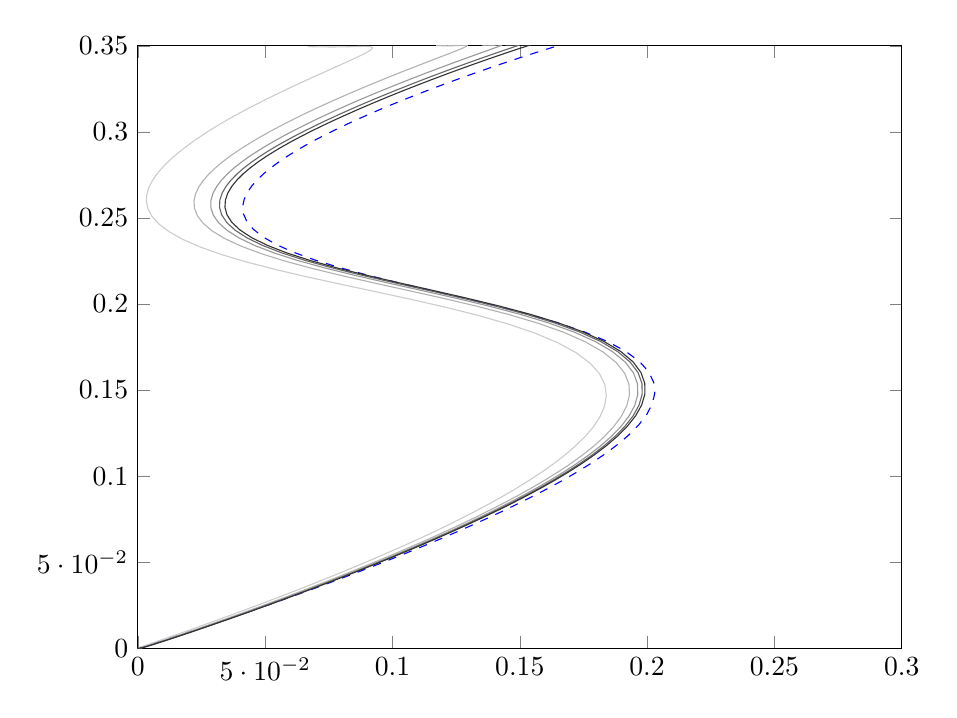
\begin{tikzpicture}

\begin{axis}[%
width=0.8\columnwidth,
height=0.630967741935484\columnwidth,
scale only axis,
xmin=0,
xmax=0.3,
ymin=0,
ymax=0.35
]
\addplot [
color=blue,
dashed,
forget plot
]
table[row sep=crcr]{
-1.22568529189217e-17 1.70219232680293e-47\\
-1.22078040529282e-17 2.17466204815869e-20\\
1.24930069097586e-15 5.59329658828069e-16\\
4.31962537102899e-13 1.9152423618868e-13\\
2.51770978879146e-11 1.11631432791867e-11\\
5.55015544523879e-10 2.46106431437956e-10\\
6.60280135771012e-09 2.9283319802688e-09\\
5.12320770129383e-08 2.27281407753508e-08\\
2.90255123674167e-07 1.28827401032052e-07\\
1.29124388293531e-06 5.73511237251698e-07\\
4.73949589296885e-06 2.10713748978966e-06\\
1.48681255318932e-05 6.6189380207418e-06\\
4.09129882041033e-05 1.82444393148059e-05\\
0.000100718153544017 4.50090857862532e-05\\
0.000225245856791989 0.000100919801590805\\
0.000463240655356511 0.000208196459707293\\
0.000884823147305501 0.000399120180670242\\
0.00158255610123486 0.000716854697447387\\
0.00266870907570527 0.00121464755420377\\
0.0042680934828865 0.00195306659807664\\
0.00650682428145541 0.00299533100932766\\
0.00949841893898853 0.00440125030957139\\
0.0133294488642299 0.00622065804358311\\
0.0180472586508033 0.00848740810159894\\
0.0236519674180277 0.0112149390444555\\
0.0300941529569334 0.0143941271208937\\
0.0372785249971626 0.0179937242124732\\
0.0450728081170337 0.0219632243456565\\
0.0533202318837492 0.0262376267222215\\
0.0618536166580361 0.0307433345872289\\
0.0705090712117028 0.0354043703208843\\
0.0791376965311413 0.0401481768418987\\
0.0876142690996799 0.0449104641836341\\
0.0958424961170963 0.0496387890730672\\
0.10375696557487 0.0542947727843779\\
0.111322280599518 0.0588550337458356\\
0.118530050316482 0.06331102120878\\
0.125394431996405 0.0676679861084513\\
0.131946828905364 0.0719433270169786\\
0.138230198729659 0.0761645191587581\\
0.144293265660084 0.0803667887860157\\
0.150184789161511 0.084590646654827\\
0.155947944238694 0.0888793518508938\\
0.161614820549927 0.0932763463165637\\
0.167201052648133 0.0978226842719481\\
0.172700648861156 0.102554481146252\\
0.178081188148765 0.107500424919056\\
0.183279696817351 0.112679429291778\\
0.188199689821794 0.11809856122523\\
0.192710046988842 0.123751440482291\\
0.196646565585241 0.12961737738435\\
0.199817148084927 0.135661573700226\\
0.202011400876493 0.141836677658674\\
0.20301387722613 0.148085506344443\\
0.202619789967853 0.154344644220661\\
0.20065273345486 0.160548886433011\\
0.196983021746862 0.166636203811203\\
0.191544736744952 0.172552738672092\\
0.184349409899893 0.178257268594913\\
0.175494381526898 0.183724581129977\\
0.165164317442443 0.188947295992029\\
0.153625080784607 0.193935846625374\\
0.1412100661361 0.198716567169214\\
0.12830006671719 0.203328087323888\\
0.115298606077758 0.207816473182085\\
0.10260527646616 0.212229725482657\\
0.0905898807700316 0.216612327368361\\
0.079570030652499 0.221000508160764\\
0.0697943393352088 0.225418764413873\\
0.0614325578259062 0.229877979341309\\
0.0545730774278078 0.234375244026284\\
0.0492273137352959 0.238895250492305\\
0.0453397371877769 0.243412935431724\\
0.0428018209176867 0.247896930561529\\
0.0414679809317703 0.252313332254143\\
0.0411716730700138 0.25662933480681\\
0.0417402386729666 0.260816396765839\\
0.0430079265640447 0.264852853167071\\
0.0448258671359753 0.268725657669276\\
0.0470681659059565 0.272431034965027\\
0.0496347242551211 0.275974250701863\\
0.0524515935766653 0.279368747748684\\
0.0554695907154709 0.282634858417776\\
0.0586617700544091 0.285798252905515\\
0.0620201947143181 0.288888235420426\\
0.0655523003124128 0.291935958228636\\
0.0692770158504934 0.294972594140621\\
0.0732207080290693 0.298027491449363\\
0.0774129544020573 0.301126332090716\\
0.0818821323091202 0.304289323201106\\
0.086650838109129 0.307529473239184\\
0.0917312255322955 0.310851034404806\\
0.0971204675308709 0.314248229434997\\
0.102796687767279 0.317704416545961\\
0.108715848493778 0.321191871765943\\
0.114810181592199 0.324672370955634\\
0.120988762173356 0.328098721508834\\
0.127140705706413 0.3314173160038\\
0.133141194808927 0.33457165455712\\
0.138860120113893 0.33750661939838\\
0.14417260737948 0.340173109510588\\
0.148970203575231 0.342532494031226\\
0.15317114157554 0.344560265930261\\
0.156728025765686 0.346248311683806\\
0.159631560364095 0.347605376663323\\
0.16190957122079 0.348655584952959\\
0.163621436389131 0.349435214610502\\
0.164848937801264 0.349988255460754\\
0.165685237911466 0.350361500346063\\
0.166223974647865 0.350599977591089\\
0.166550272189824 0.350743403168433\\
0.166734851771187 0.350824053127807\\
0.166831595215191 0.350866113799758\\
0.166878121826248 0.350886259282569\\
0.166898406741448 0.350895013534916\\
0.166906302339804 0.350898412202254\\
0.16690899217171 0.35089956776726\\
0.166909773384699 0.350899902896113\\
0.166909959992641 0.350899982867216\\
0.166909994843181 0.350899997792469\\
0.166909999566499 0.350899999814467\\
0.166909999980335 0.350899999991584\\
0.166909999999663 0.350899999999856\\
0.166909999999999 0.3509\\
0.16691 0.3509\\
0.16691 0.3509\\
};
\addplot [
color=white!80!black,
solid,
forget plot
]
table[row sep=crcr]{
-1.22568529189217e-17 1.70219232680293e-47\\
3.25274463507264e-06 8.35905362814104e-08\\
1.23717401990733e-05 6.51809556987925e-07\\
2.60782198962572e-05 2.10499070948953e-06\\
4.3092311772854e-05 4.74258914527822e-06\\
6.21318876894655e-05 8.7637958130708e-06\\
8.19125001256813e-05 1.42692959778432e-05\\
0.000101156688969535 2.12681872858731e-05\\
0.000118643983994053 2.97049649157848e-05\\
0.000133386193364771 3.95467615229986e-05\\
0.00014510004883005 5.10128278393354e-05\\
0.0001552465101183 6.5075416432896e-05\\
0.000168952051477796 8.43854757627399e-05\\
0.000198041564834851 0.000114740042164133\\
0.00026513772561189 0.000167083224948609\\
0.000408333337430968 0.000259824989119074\\
0.000685436662127054 0.000421023858453292\\
0.00117641921404975 0.000689800526123193\\
0.0019826628090404 0.0011163219128708\\
0.00322202345439749 0.00175987161326193\\
0.00501956323556232 0.00268488373870233\\
0.00749484404363355 0.0039552731473001\\
0.0107476267088559 0.00562781764097272\\
0.0148443828740994 0.00774561614639042\\
0.0198080260882525 0.0103326877885853\\
0.0256126991972536 0.0133905843814564\\
0.0321844810802911 0.0168975212907577\\
0.0394077642119747 0.0208100876679215\\
0.0471360843591468 0.0250671836813051\\
0.0552055623017432 0.0295955336269499\\
0.0634489323010695 0.0343159814489065\\
0.0717083475272989 0.0391497861089964\\
0.0798456440508612 0.0440242623581138\\
0.0877493512990643 0.0488773077339653\\
0.0953383119334656 0.0536605715857425\\
0.102562219474309 0.0583412200179673\\
0.109399655339149 0.0629024072076402\\
0.115854312001125 0.0673426650555623\\
0.121950058891251 0.0716744673315447\\
0.127725389733361 0.075922219782685\\
0.133227633162548 0.0801198897574413\\
0.138507154146251 0.0843084353295575\\
0.143611650722376 0.0885331395891004\\
0.148580574700905 0.0928409108464387\\
0.15343968194199 0.0972775796199095\\
0.158195747221979 0.101885211071146\\
0.16283155730666 0.106699458175359\\
0.16730141867135 0.111747006834142\\
0.171527575073714 0.117043208571809\\
0.175398110794516 0.122590056608926\\
0.17876709519038 0.128374731727528\\
0.181457870007442 0.13436901784707\\
0.183270418807971 0.140529933609352\\
0.183992840168584 0.1468017196852\\
0.183415811647512 0.153118883204305\\
0.181349255134415 0.159410354303193\\
0.177640391773053 0.165604747985411\\
0.172191559796912 0.171636409453042\\
0.164975852452944 0.177451555876\\
0.156048491179281 0.183013478959773\\
0.145551999572995 0.188305754446059\\
0.133713873420574 0.193332875414501\\
0.120836446899598 0.198118387394409\\
0.107279687175711 0.202701044925459\\
0.0934385122850055 0.207129644586298\\
0.0797168904764897 0.211457183163945\\
0.0665013860742654 0.215734973676006\\
0.0541368781104964 0.22000733245879\\
0.0429068577808264 0.224307382025773\\
0.033020059316166 0.22865437252083\\
0.0246043139118881 0.233052722129095\\
0.0177075894370749 0.237492749893384\\
0.0123053407655547 0.241952864909341\\
0.00831266795198405 0.246402818708713\\
0.00559943353492465 0.250807543394727\\
0.00400643982833325 0.255131090794861\\
0.00336099531970944 0.259340261583538\\
0.00349094963575494 0.263407694601951\\
0.00423632700566043 0.267314287640521\\
0.00545739698604056 0.271050520324513\\
0.00703909360281847 0.274616713655985\\
0.00889256053514898 0.278022468888926\\
0.0109545952245223 0.281285525081238\\
0.0131856580959084 0.284430233952467\\
0.0155669691751959 0.28748580297281\\
0.018097061806758 0.290484411403001\\
0.0207880223567336 0.293459265457746\\
0.0236615294186096 0.296442631788672\\
0.0267447249692657 0.29946387492171\\
0.0300659091430229 0.30254752444948\\
0.0336500541993982 0.305711411122957\\
0.0375141841333209 0.308964936070606\\
0.0416627620032532 0.312307571339502\\
0.0460833573873633 0.315727727789735\\
0.0507430103470991 0.319202160247643\\
0.0555858324175085 0.322696098963651\\
0.0605324459864692 0.326164288076076\\
0.0654818150895609 0.32955306358398\\
0.0703158276701347 0.332803506928079\\
0.0749066424601935 0.335855565592948\\
0.0791263436331281 0.338652851337519\\
0.0828579300985524 0.341147637015078\\
0.086006219944052 0.343305417717783\\
0.0885070089368458 0.345108336437797\\
0.0903329042299405 0.34655685170897\\
0.0914947162488735 0.34766926934375\\
0.0920380775007132 0.348479140774549\\
0.0920358866418595 0.349030952794802\\
0.0915779982342309 0.349374872001687\\
0.0907600654711163 0.349561458970446\\
0.0896734678021941 0.349637195188974\\
0.0883978262579761 0.349641406227386\\
0.0869968669564486 0.349604803855963\\
0.0855175674063735 0.349549511893666\\
0.0839918507219313 0.349490176744121\\
0.0824397444046635 0.349435647523352\\
0.0808729297318141 0.349390745172857\\
0.0792978877849283 0.349357781483348\\
0.0777182414268251 0.349337669415243\\
0.076136245249234 0.349330621539781\\
0.0745535944675742 0.349336526488321\\
0.0729717944868774 0.349355120123051\\
0.0713922993651467 0.349386049440274\\
0.0698165526897378 0.34942889134331\\
0.068245996566624 0.349483156689842\\
0.0666820730088789 0.349548290832413\\
};
\addplot [
color=white!70!black,
solid,
forget plot
]
table[row sep=crcr]{
-1.22568529189217e-17 1.70219232680293e-47\\
6.93129473689265e-06 9.64767466645037e-08\\
2.7053728010589e-05 7.53393712416719e-07\\
5.90241087723482e-05 2.43942373846901e-06\\
0.000101498155661405 5.51343408114195e-06\\
0.000153129376081493 1.02251741061884e-05\\
0.000212569038951388 1.67171588199604e-05\\
0.000278475522813864 2.50317808145982e-05\\
0.000349564364216304 3.51385921991254e-05\\
0.000424783594102553 4.70220206280164e-05\\
0.000503786426983947 6.09116511278121e-05\\
0.000587970596547154 7.77844535591212e-05\\
0.000682399652245789 0.000100292595867371\\
0.000798835848869633 0.000134233849753492\\
0.000959839481982006 0.000190556312586955\\
0.00120344120098727 0.000287681051323386\\
0.00158738733147519 0.000453687794298591\\
0.00219158773190882 0.000727729550523115\\
0.00311736305544096 0.00116001496346112\\
0.00448250910290361 0.00180987440428384\\
0.00641202948157397 0.00274178773012311\\
0.00902543036526304 0.00401970807708507\\
0.0124224207575113 0.00570043852896392\\
0.0166694253808309 0.00782708640457289\\
0.0217893165013838 0.0104236601922089\\
0.0277562016851992 0.0134916813674616\\
0.0344961305342789 0.0170093156475479\\
0.0418934719326902 0.0209330844092612\\
0.0498017431838193 0.025201803884487\\
0.0580570510257657 0.0297421012468949\\
0.0664921193903008 0.0344747144410509\\
0.0749490943067283 0.0393207933494284\\
0.083289807743699 0.0442075475846333\\
0.0914027883802557 0.0490727809439252\\
0.0992068821701957 0.053868067178828\\
0.106651790765752 0.0585605198516327\\
0.113716109160424 0.0631332660419391\\
0.120403549051503 0.0675848357938546\\
0.12673800451864 0.0719277239249715\\
0.132757998825081 0.0761863763987518\\
0.138510894368985 0.0803948155499262\\
0.144047093460022 0.0845940647197951\\
0.149414334532967 0.0888294783218773\\
0.154652112482077 0.0931480382373108\\
0.159786228723888 0.0975956474153343\\
0.164823505971776 0.102214439249045\\
0.169746781305514 0.107040127859175\\
0.174510413938733 0.1120994503015\\
0.179036702853095 0.11740779612371\\
0.183213790070021 0.122967179842902\\
0.186895805137288 0.128764782568114\\
0.1899061521658 0.134772362639757\\
0.192044878582981 0.1409468819141\\
0.193100147022395 0.1472324882047\\
0.19286269715242 0.153563556499437\\
0.19114250810376 0.159868847403178\\
0.187786850523484 0.166076780850869\\
0.182698103454159 0.172121506524738\\
0.175849394842952 0.177949080546467\\
0.167295979727899 0.183522700154989\\
0.157180417585707 0.188825927304757\\
0.145730241246288 0.193863312442234\\
0.133247818825882 0.198658504269697\\
0.120093144190204 0.203250378202201\\
0.106661152660102 0.207687847535028\\
0.0933558199927957 0.212024008470429\\
0.0805637088347397 0.216310250212964\\
0.0686296882127832 0.220590940806223\\
0.0578372317943576 0.224899231308802\\
0.0483950494317936 0.229254379779297\\
0.0404309416589472 0.233660794691578\\
0.0339928399182604 0.238108770890859\\
0.029056157412647 0.242576681968768\\
0.0255359478476862 0.247034235902087\\
0.0233020233782072 0.25144631659818\\
0.022195132642067 0.255776926658629\\
0.0220425280052933 0.259992820280044\\
0.0226720014664253 0.264066596454024\\
0.0239235191055781 0.267979123522436\\
0.0256572927278969 0.271720864841182\\
0.0277581997534111 0.275292139685674\\
0.0301373289229437 0.278702562031931\\
0.0327314247052732 0.281969896717172\\
0.0355008966451315 0.285118531913417\\
0.0384269160159032 0.288177719212875\\
0.0415079695590667 0.29117968640564\\
0.0447560992523834 0.294157689412887\\
0.0481929416503832 0.297144042766935\\
0.0518455992455894 0.300168154376497\\
0.0557423354994946 0.303254590408189\\
0.0599080890900244 0.306421209410366\\
0.0643598537911934 0.309677429863546\\
0.0691020660270022 0.313022729303285\\
0.0741222724777841 0.31644551101468\\
0.0793874940891376 0.319922508214131\\
0.0848418269794431 0.3234189148495\\
0.0904058815988261 0.326889423920117\\
0.0959786131876827 0.330280306170263\\
0.101441903661408 0.333532565762175\\
0.106667908232484 0.336586064933916\\
0.111528710145165 0.339384328716674\\
0.115907310598752 0.341879550643571\\
0.119708534372898 0.344037164229383\\
0.12286818970643 0.345839278347961\\
0.125358902890373 0.347286351236394\\
0.127191509935881 0.348396722962202\\
0.128411673995255 0.349204008280944\\
0.129092327454437 0.349752776234616\\
0.129323359924559 0.350093282717987\\
0.129200459903221 0.350276173935389\\
0.128815042047515 0.350348005584898\\
0.128246762583773 0.350348161750893\\
0.127559383036323 0.350307395802087\\
0.126799916704839 0.350247857240857\\
0.126000322945996 0.350184204555702\\
0.1251806659329 0.350125288184074\\
0.124352663973483 0.350075922368641\\
0.123522835457299 0.350038406444803\\
0.122694840758248 0.350013636784894\\
0.12187097212178 0.350001806250653\\
0.12105296251271 0.350002781183144\\
0.120242355145558 0.350016272815784\\
0.119440641921753 0.350041901264811\\
0.11864930428768 0.350079214324527\\
0.117869822211852 0.350127691516173\\
0.117103675565859 0.350186744625179\\
};
\addplot [
color=lightgray!80!black,
solid,
forget plot
]
table[row sep=crcr]{
-1.22568529189217e-17 1.70219232680293e-47\\
8.24119022140355e-06 1.00732406791694e-07\\
3.22818627429921e-05 7.86940656335505e-07\\
7.07559323208588e-05 2.54986090125147e-06\\
0.000122296228331723 5.76797064381405e-06\\
0.00018553338427912 1.07077012838254e-05\\
0.000259095822954879 1.75253638232066e-05\\
0.000341619118787306 2.62743262033844e-05\\
0.000431796062051802 3.69323957213372e-05\\
0.000528552011866369 4.94896975186751e-05\\
0.000631517600857057 6.41792322979517e-05\\
0.000742068082289762 8.19795699039566e-05\\
0.000865244631480491 0.000105543401475197\\
0.00101278723256497 0.000140668999415314\\
0.00120723400539919 0.000198306249405875\\
0.00148659350872234 0.000296880649727077\\
0.00190859005869599 0.000464480052181126\\
0.002553111603022 0.000740269632660934\\
0.00352145704973565 0.00117447363800878\\
0.00493140077336401 0.00182643993469807\\
0.00690792553655244 0.00276066560601727\\
0.00957051760868816 0.00404111845209194\\
0.013018867428092 0.00572461167681009\\
0.0173193828571617 0.00785425676069301\\
0.0224949212787883 0.0104540595927566\\
0.0285195774988574 0.0135255320009586\\
0.035319390500034 0.017046823099313\\
0.0427787205908372 0.0209744310901322\\
0.0507510783541073 0.0252471431363759\\
0.0590725654150967 0.0297915525019845\\
0.0675759019452456 0.0345283599239281\\
0.0761032313718057 0.0393786768622851\\
0.0845163841555275 0.0442696758156739\\
0.0927038886619868 0.0491391274533087\\
0.100584591960087 0.0539385788040041\\
0.108108198522499 0.0586351248731017\\
0.115253308079248 0.0632118832043138\\
0.122023639052197 0.0676673832532119\\
0.128443094156398 0.0720141273595286\\
0.134550207016313 0.076276575782572\\
0.140392351886249 0.0804887703534101\\
0.146019944204992 0.0846917575060123\\
0.151480736630151 0.0889309168345366\\
0.156814239248724 0.0932532561315467\\
0.162046269569075 0.0977047037845897\\
0.167183667267311 0.102327417068251\\
0.172209287258199 0.107157131409542\\
0.177077507480326 0.112220601573851\\
0.181710646551086 0.117533230120374\\
0.18599686704668 0.123097038618307\\
0.189790319960976 0.128899207779441\\
0.192914431638598 0.134911486360631\\
0.195169272283309 0.141090815579626\\
0.196343027377081 0.147381309838045\\
0.196226458744299 0.153717296801278\\
0.194629565937674 0.160027476514049\\
0.191399637271586 0.166240199323007\\
0.18643906636242 0.172289545207232\\
0.179720993560132 0.178121512882846\\
0.171300685919523 0.183699265895567\\
0.16132071575316 0.189006361231044\\
0.15000862915004 0.194047369705262\\
0.137666806389296 0.198845976718071\\
0.124655250930212 0.203441100722334\\
0.11136890434015 0.207881696624692\\
0.0982117451440555 0.212220896144709\\
0.0855703354850615 0.216510115804387\\
0.0737895409198586 0.220793742315416\\
0.0631528289654475 0.225104937212302\\
0.0538689008840692 0.229462961720491\\
0.0460655463836004 0.233872221219448\\
0.0397906840306257 0.238323002294295\\
0.0350197122887116 0.242793666223433\\
0.0316676684619934 0.247253905761631\\
0.0296043468694794 0.251668587890903\\
0.0286704771406535 0.256001697867092\\
0.0286932917590319 0.260219973468202\\
0.0295005622973088 0.264295999581883\\
0.0309322342141809 0.268210634111924\\
0.0328484988224416 0.271954334638874\\
0.0351342134438643 0.275527419817031\\
0.0377004473008033 0.278939508125996\\
0.0404839260303129 0.282208373537663\\
0.0434450410789383 0.285358417140878\\
0.0465649463701479 0.288418906155873\\
0.0498421120540551 0.291422085547991\\
0.0532885643012866 0.294401228807807\\
0.0569259246939338 0.297388667359027\\
0.060781281661924 0.300413824369689\\
0.0648828856070467 0.303501278808989\\
0.0692556632508983 0.306668898869657\\
0.0739165976105503 0.309926108924857\\
0.0788701156320308 0.313272388148497\\
0.0841037558484537 0.316696136786902\\
0.0895845324026466 0.320174080001135\\
0.0952565359222051 0.323671398441293\\
0.101040372596916 0.327142766524831\\
0.106834994514794 0.330534431396352\\
0.112522281411398 0.333787369354094\\
0.117974387199522 0.336841411957749\\
0.123063394734693 0.339640053057411\\
0.127672305965782 0.342135457664629\\
0.131705947986898 0.344293037104961\\
0.135100133412516 0.346094887844805\\
0.137827495291969 0.3475414677501\\
0.139898878703717 0.348651128804713\\
0.141359957684072 0.349457508011248\\
0.142283676615549 0.350005203379756\\
0.142759937586791 0.350344502272953\\
0.142884441669828 0.350526081058766\\
0.142748616062309 0.350596521548441\\
0.14243212952282 0.350595228378737\\
0.141998756175451 0.350552969484934\\
0.141495522047665 0.350491903311688\\
0.140954399376044 0.350426692491499\\
0.140395465359062 0.350366187815311\\
0.13983045145243 0.350315201062375\\
0.139265889288576 0.350276027090483\\
0.138705452554353 0.350249556355617\\
0.138151446857674 0.350235974722749\\
0.137605618559151 0.350235140647284\\
0.13706952429002 0.350246756673952\\
0.136544669380156 0.350270433458172\\
0.136032548709625 0.350305708569233\\
0.135534655681571 0.350352050539719\\
0.135052483600492 0.350408859401613\\
};
\addplot [
color=gray!80!black,
solid,
forget plot
]
table[row sep=crcr]{
-1.22568529189217e-17 1.70219232680293e-47\\
8.92977877512262e-06 1.02875256139306e-07\\
3.50302073670603e-05 8.03832204998465e-07\\
7.6923181451443e-05 2.6054666526772e-06\\
0.000133229513849615 5.89612735388159e-06\\
0.000202567829414407 1.09506412435071e-05\\
0.000283554556587495 1.79322606298721e-05\\
0.000374813297083546 2.68998738572252e-05\\
0.000475024898264518 3.78354390567461e-05\\
0.00058310281472824 5.07319460217592e-05\\
0.000698665821066556 6.58241162764799e-05\\
0.000823077365168913 8.40913381849907e-05\\
0.000961366872516901 0.000108186603085048\\
0.00112526263206191 0.000143908514171362\\
0.0013372911192877 0.000202208001417812\\
0.00163544929455634 0.000301513027909894\\
0.00207744991934694 0.000469915878014372\\
0.00274316943818554 0.00074658831036123\\
0.00373389534015586 0.0011817629856139\\
0.00516739074226722 0.00183479720468099\\
0.00716862744585325 0.00277019737138397\\
0.00985708124108685 0.00405193928677507\\
0.0133324327779902 0.00573684179051188\\
0.017661081015106 0.00786801888227079\\
0.0228658754619511 0.0104694754201866\\
0.0289209041629876 0.0135427184867887\\
0.0357522004656874 0.0170658887717894\\
0.0432441201229809 0.0209954725658302\\
0.0512501701454335 0.0252702419822597\\
0.0596064494404405 0.0298167726496399\\
0.0681456761811332 0.0345557458973301\\
0.0767099924117116 0.0394082531059054\\
0.0851612277883653 0.0443014473555745\\
0.0933879105000287 0.0491730819721281\\
0.101308888187009 0.0539746899928377\\
0.108873866784702 0.0586733567120258\\
0.116061448486722 0.0632521946938633\\
0.122875355216972 0.0677097331068654\\
0.12933949419109 0.0720584782550339\\
0.135492404436783 0.0763228979085512\\
0.141381466394777 0.0805370441269593\\
0.147057102358845 0.0847419754453117\\
0.152567072418053 0.0889830846373902\\
0.157950894604189 0.0933073930400802\\
0.163234394848169 0.0977608423175764\\
0.168424421712857 0.102385602185229\\
0.173503839465477 0.10721741914209\\
0.178427035872348 0.11228305712342\\
0.183116339864578 0.11759792538159\\
0.187459924821671 0.123164049044482\\
0.191311953014686 0.128968608470596\\
0.194495862483409 0.134983347244226\\
0.196811735414456 0.141165195614265\\
0.198047769311679 0.147458250317859\\
0.197994737657609 0.153796814064669\\
0.196462650751454 0.160109555005934\\
0.193298806206009 0.166324786867196\\
0.188405605310313 0.172376552959401\\
0.18175619494662 0.178210821802491\\
0.173405848500447 0.183790739213434\\
0.163497145047472 0.189099859549082\\
0.152257637664544 0.194142764317839\\
0.139989713044845 0.19894315820053\\
0.12705337971325 0.203539982274023\\
0.113843582544761 0.207982213333711\\
0.100764301543973 0.212323001802113\\
0.0882020986142179 0.216613778612594\\
0.0765018375125098 0.220898940359292\\
0.0659469825469476 0.22521165416738\\
0.0567462304884415 0.229571183020556\\
0.049027365378689 0.233981930769087\\
0.0428382990414638 0.238434179751384\\
0.0381544222191173 0.242906284861195\\
0.0348907636219798 0.247367930928288\\
0.0329171082219877 0.251783976100636\\
0.0320741756852476 0.256118396564673\\
0.0321891880715997 0.260337921502582\\
0.0330899062427278 0.264415128410756\\
0.0346162648409108 0.2683308697187\\
0.036628444427112 0.272075599975723\\
0.0390112917748274 0.275649637507928\\
0.0416758658592514 0.279062603155282\\
0.0445588824278458 0.282332275679604\\
0.0476207234201685 0.285483062942925\\
0.0508425336436436 0.288544240358539\\
0.0542227745293641 0.291548061892158\\
0.0577734639401573 0.294527810235089\\
0.0615162155887227 0.29751582564768\\
0.0654781105140704 0.300541539268275\\
0.069687392254882 0.303629536735988\\
0.0741689812505039 0.306797691244088\\
0.0789398548670954 0.310055430185055\\
0.0840044350727047 0.31340223350734\\
0.0893502561221372 0.316826499765939\\
0.0949443285860845 0.320304949788047\\
0.10073074020827 0.323802757130865\\
0.106630094939127 0.327274586340627\\
0.112541343206658 0.330666672055047\\
0.118346363594059 0.333919975828261\\
0.123917309320733 0.336974313002536\\
0.129126263024408 0.339773160953013\\
0.133856227032223 0.342268669620473\\
0.138012029638276 0.344426238592833\\
0.141529485741297 0.346227957742641\\
0.144381231929687 0.347674284668092\\
0.146578118038222 0.348783577541131\\
0.148165823818506 0.349589484978445\\
0.149217299956915 0.350136620133057\\
0.14982245510157 0.350475286822565\\
0.15007699693636 0.350656177185017\\
0.150072359252929 0.350725886677099\\
0.149888217398158 0.350723830665718\\
0.149588352117699 0.350680784680134\\
0.149219796125307 0.350618911814269\\
0.148814528421328 0.350552876839747\\
0.14839263304238 0.350491530705835\\
0.147965848345104 0.350439683880285\\
0.147540712911789 0.350399628860669\\
0.147120907415342 0.350372252995834\\
0.146708744475372 0.350357738484599\\
0.146305977481483 0.35035593965763\\
0.145914170104769 0.350366554521367\\
0.145534834721014 0.350389188795593\\
0.145169473258873 0.350423374720786\\
0.1448195861705 0.35046857510784\\
0.144486673808429 0.350524183873566\\
};
\addplot [
color=darkgray!80!black,
solid,
forget plot
]
table[row sep=crcr]{
-1.22568529189217e-17 1.70219232680293e-47\\
9.3599787039213e-06 1.0417101912332e-07\\
3.67472565733727e-05 8.14046240397971e-07\\
8.07762283287326e-05 2.63908981594335e-06\\
0.000140060207390276 5.97361816027719e-06\\
0.000213210324072626 1.10975329272605e-05\\
0.000298835521074842 1.81782813127163e-05\\
0.000395551927675744 2.72780870527299e-05\\
0.000502032937133339 3.83814155625667e-05\\
0.000617184573577938 5.14829869834302e-05\\
0.00074061820980064 6.68185639616807e-05\\
0.000873689924463659 8.5368036054316e-05\\
0.00102142180835642 0.000109784593732231\\
0.00119553484998007 0.000145867077780254\\
0.00141854825650836 0.000204567118240015\\
0.00172845174930132 0.000304314279952965\\
0.0021829508785694 0.000473203690687496\\
0.00286191490956714 0.000750411307059446\\
0.00386662420340855 0.0011861751429198\\
0.00531483484716441 0.00183985850187608\\
0.00733151179290929 0.00277597373183081\\
0.0100361242771989 0.00405850176585805\\
0.0135283468221219 0.00574426510863267\\
0.0178745728054188 0.00787637948475917\\
0.0230976467956264 0.0104788492611891\\
0.0291716525890287 0.0135531787042616\\
0.0360226199889105 0.0170775033788272\\
0.043534901880865 0.021008302256862\\
0.051562003026155 0.0252843381546641\\
0.0599400206208809 0.0298321757695653\\
0.0685016715802959 0.0345724843748974\\
0.0770890970779875 0.0394263428602883\\
0.0855641262624378 0.0443208922158884\\
0.0938152872071621 0.0491938749645788\\
0.101761427903042 0.0539968154279506\\
0.109352255190543 0.0586967928535431\\
0.116566372790718 0.0632769167100027\\
0.123407504800645 0.067735715997117\\
0.129899561230249 0.0720856995007324\\
0.136081084463359 0.0763513396822957\\
0.141999458784845 0.0805666949831835\\
0.147705110750004 0.0847728314821394\\
0.153245805070229 0.0890151501618397\\
0.158661064721878 0.0933406807870793\\
0.163976720881216 0.0977953732740882\\
0.169199627649344 0.102421405060018\\
0.174312655125908 0.107254529503681\\
0.179270197209958 0.112321516206356\\
0.183994589272221 0.117637778535721\\
0.188374011440659 0.123205343775658\\
0.192262633033297 0.129011391998196\\
0.195483899399841 0.135027663494474\\
0.197837900217713 0.141211081605555\\
0.199112840506493 0.147505731986089\\
0.199099501037313 0.153845901717464\\
0.197607898828365 0.160160238997701\\
0.194485337306686 0.166377034653828\\
0.18963422255999 0.172430309075094\\
0.183027705557095 0.178266011906733\\
0.174721063644686 0.183847277881476\\
0.164856880130506 0.189157659706088\\
0.153662712464837 0.19420174556224\\
0.141440951356884 0.199003252172211\\
0.128551608506045 0.20360113474741\\
0.115389630864249 0.208044383764832\\
0.102358999371317 0.212386161346023\\
0.0898462757916453 0.216677907450459\\
0.0781963227686839 0.220964024876747\\
0.0676926026164741 0.225277684279662\\
0.0585438093107243 0.2296381497825\\
0.0508777233642002 0.234049824323025\\
0.0447422523995665 0.238502987628501\\
0.040112782347364 0.24297599064265\\
0.0369043365614955 0.247438513277933\\
0.0349866941872291 0.251855408191103\\
0.0342005686790319 0.256190645923996\\
0.0343731755972173 0.260410950304008\\
0.0353322691237018 0.264488894219923\\
0.0369177771540226 0.268405326686834\\
0.0389898735413398 0.272150700362392\\
0.0414333984769443 0.275725333366954\\
0.0441594045403562 0.279138848012056\\
0.0471046013052596 0.282409026046797\\
0.0502293647751702 0.28556027955736\\
0.053514834064677 0.288621889065871\\
0.0569594651593455 0.291626114148557\\
0.0605752707329631 0.294606243229344\\
0.0643838595829539 0.297594622070293\\
0.0684123081321 0.300620686766432\\
0.0726888556329081 0.3037090270971\\
0.0772384186018462 0.306877519348699\\
0.0820779708770266 0.310135592764979\\
0.0872119313191577 0.313482727739413\\
0.0926278315128938 0.316907321728181\\
0.0982926797997083 0.320386092806208\\
0.104150562123465 0.32388421005322\\
0.110122081036359 0.327356331801865\\
0.116106185928705 0.330748684830497\\
0.121984754661522 0.334002221438116\\
0.12762994001709 0.337056746794087\\
0.132913824491634 0.339855727942772\\
0.137719410642107 0.342351305374223\\
0.141951527505355 0.344508871310043\\
0.145545991400554 0.346310511470982\\
0.148475441121506 0.347756683255383\\
0.150750729470393 0.348865748667293\\
0.152417539767093 0.349671363543548\\
0.153548826635592 0.350218150460284\\
0.154234502822518 0.350556423476957\\
0.154570280143574 0.350736884546155\\
0.154647596510981 0.350806137613783\\
0.154546131387969 0.350803604718214\\
0.154329669656292 0.35076006610554\\
0.154045248205047 0.350697687752151\\
0.153724850257181 0.350631135749437\\
0.153388564117416 0.350569261134261\\
0.153048132449003 0.350516873548681\\
0.152710098170926 0.350476264014004\\
0.15237814631509 0.350448317940478\\
0.152054593875948 0.350433215243187\\
0.151741198628649 0.350430807686562\\
0.151439528636546 0.350440790456397\\
0.151151100671428 0.350462766207533\\
0.150877421059584 0.350496263873815\\
0.150619994651039 0.350540742717994\\
0.150380326195567 0.350595592866864\\
};
\end{axis}
\end{tikzpicture}%}
\caption{Convergence of $\alg$ to the reference table tennis trajectory for the joints 5, 6 and 7}
\label{wILCTrajectoryTT}
\end{figure}

\begin{figure}
\begingroup
%\tikzset{every picture/.style={scale=0.8}}%
\scalebox{0.5}{% This file was created by matlab2tikz v0.4.4 running on MATLAB 8.2.
% Copyright (c) 2008--2013, Nico Schlömer <nico.schloemer@gmail.com>
% All rights reserved.
% 
% The latest updates can be retrieved from
%   http://www.mathworks.com/matlabcentral/fileexchange/22022-matlab2tikz
% where you can also make suggestions and rate matlab2tikz.
% 
\begin{tikzpicture}

\begin{axis}[%
width=5.14083333333333in,
height=3.48638888888889in,
scale only axis,
xmin=1,
xmax=5,
xtick={1, 2, 3, 4, 5},
xlabel={Episodes},
ymode=log,
ymin=0.01,
ymax=10,
yminorticks=true,
ylabel={Root Mean Squared Error (RMS)},
title={Comparison of ILC to two RL approaches},
legend style={draw=black,fill=white,legend cell align=left}
]
\addplot [
color=black,
dashed,
line width=1.0pt
]
table[row sep=crcr]{
1 0.550705874707667\\
2 0.152998198590581\\
3 0.0758718186428609\\
4 0.0488997673400057\\
5 0.036794112098251\\
};
\addlegendentry{wILC};

\addplot [
color=black,
dotted,
line width=1.0pt
]
table[row sep=crcr]{
1 3\\
2 1.5\\
3 2\\
4 1.6\\
5 0.5\\
};
\addlegendentry{REPS};

\addplot [
color=black,
dash pattern=on 1pt off 3pt on 3pt off 3pt,
line width=1.0pt
]
table[row sep=crcr]{
1 2.4\\
2 0.8\\
3 1.8\\
4 0.4\\
5 0.3\\
};
\addlegendentry{PI2};

\end{axis}

\begin{axis}[%
width=6.63333333333333in,
height=4.27777777777778in,
scale only axis,
xmin=0,
xmax=1,
ymin=0,
ymax=1,
hide axis,
axis x line*=bottom,
axis y line*=left
]
\addplot [
color=black,
solid,
line width=0.0pt,
mark=square*,
mark options={solid,fill=black,draw=white},
forget plot
]
table[row sep=crcr]{
0.5 0.987012987012987\\
};
\addplot [
color=black,
solid,
line width=0.0pt,
mark=square*,
mark options={solid,fill=black,draw=white},
forget plot
]
table[row sep=crcr]{
0.991624790619765 0.5\\
};
\addplot [
color=black,
solid,
line width=0.0pt,
mark=square*,
mark options={solid,fill=black,draw=white},
forget plot
]
table[row sep=crcr]{
0.5 0.012987012987013\\
};
\addplot [
color=black,
solid,
line width=0.0pt,
mark=square*,
mark options={solid,fill=black,draw=white},
forget plot
]
table[row sep=crcr]{
0.00837520938023451 0.5\\
};
\addplot [
color=black,
solid,
line width=0.0pt,
mark=square*,
mark options={solid,fill=black,draw=white},
forget plot
]
table[row sep=crcr]{
0.00837520938023451 0.987012987012987\\
};
\addplot [
color=black,
solid,
line width=0.0pt,
mark=square*,
mark options={solid,fill=black,draw=white},
forget plot
]
table[row sep=crcr]{
0.991624790619765 0.012987012987013\\
};
\addplot [
color=black,
solid,
line width=0.0pt,
mark=square*,
mark options={solid,fill=black,draw=white},
forget plot
]
table[row sep=crcr]{
0.991624790619765 0.987012987012987\\
};
\addplot [
color=black,
solid,
line width=0.0pt,
mark=square*,
mark options={solid,fill=black,draw=white},
forget plot
]
table[row sep=crcr]{
0.00837520938023451 0.012987012987013\\
};
\end{axis}
\end{tikzpicture}%}
\endgroup
\caption{The log-scale plot of convergence of \emph{wILC}. Note the slow convergence of the other stochastic RL algorithms.}
\label{ttComparison}
\end{figure}
%\section{CONCLUSION}\label{end}

% shall we put inv. dynamics eq here?
The cost functional to be minimized considers the accelerations as the quantity to be minimized. It assumes that the feedback linearization of the robot is perfect, that is the inverse dynamics model for the robot is exact. Whenever the cancellation is imperfect due to inaccurate robot control, execution error will prevent the robot from achieving the desired trajectories. Execution errors will be considered in future work.

\section{INTRODUCTION}

The opponent's court in table tennis, the net and other environmental restrictions such as walls together define a natural \emph{stability region} that is intrinsic to the game: the table tennis playing robot implementing our favorite reinforcement learning and control algorithm will lose a point if they cannot land the ball on the other side of the table. Taken in a wider sense, this stability region is a result of the redundancy in task-specification, and should be exploited as much as possible in all robotic tasks. 
% $\court$

An aspect in table tennis that strengthens this point is the uncertainty in ball estimation. As a result of limitations in the sensing hardware as well as in our simple physical models that neglect certain dynamics, the ball cannot be estimated or predicted perfectly within the workspace of the robot. In an ideal world where this could be done, exploitation of task-redundancy could indeed be relegated to a higher-level strategy, as is often done in previous works in table tennis~\cite{Muelling13}. However, whenever there is ball uncertainty, being aware and taking advantage of the stability region is critical and directly contributes to generating successful playing styles.
%  It is difficult to estimate the center of mass of the ball from image data. Small errors in position can accumulate to much larger errors in velocity estimates. Moreover, the ball is very light and some effects such as spin cannot be predicted precisely even with sophisticated modelling.

% But nobody should blame them if they land the ball precisely on a target point but only within a certain region of it: they do not have to! Even humans with very agile striking capabilities are not able to return the ball to a precise location.
% mention human studies in this aspect

In this paper, we incorporate probabilistic modeling for robust trajectory generation and come up with a new performance criterion in table tennis that exploits the game's natural stability criterion. The cost functional that we try to minimize is not \emph{certainty-equivalent} and naturally leads to \emph{cautious} strategies. Moreover it is particularly suitable for employing adaptive strategies as the robot gets more data and refines its internal models of the environment. 

Our approach involves intensive modeling of task-relevant quantities from data, e.g. ball flight, bounce models and ball-racket contact modeling. The last one especially can be hard to train from missing data. However, we keep the uncertainty of all of our models and use them also in our decision-making process. This cautious design is an asset that differentiates our approach from previous approaches (e.g. \cite{Matsushima05}, \cite{Muelling13}) that are less robust to modeling and estimation uncertainty.
% from missing data and can even be misleading when given example ball trajectories with high spin.

To summarize our reasons for introducing uncertainty and probabilistic modeling to trajectory generation in table tennis: \textit{i)} Table tennis balls are very light and cannot be estimated or predicted precisely. \textit{ii)} Racket-ball interaction is generally not known well and the elasticity of the momentum exchange differentiates it from the mirror laws used in the literature so far. \textit{iii)} The set of allowed landing point specifications in the opponent's side can be incorporated to design robust algorithms that return the ball with a higher probability, when under the influence of various effects mentioned in \textit{(i)} and \textit{(ii)}. See figure~\ref{mainIdea} for an illustration.% ref needed obviously 
% velocity dependent coefficient of restitution

% The choice of the the desired landing point of the ball on the opponent's court is generally left to a higher level strategy or policy of the robot. However in this paper we argue that landing the ball successfully on the opponent's court is the \emph{fundamental goal} in table tennis. Therefore policies or the strategies involved in striking movement generation should be combined in one unitary whole.

\begin{figure}[t!]
\center
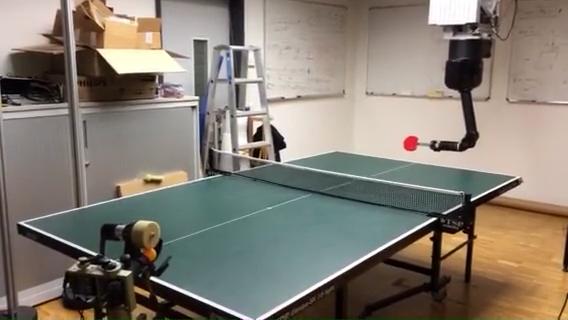
\includegraphics[scale=0.4]{robot1.png}			
\caption{Robotic table tennis setup with four cameras tracking the ball at 60 Hz. In order to return the ball to the opponent's court, we need to consider the uncertainty in ball estimation as well as in our ball-racket contact model. Introducing uncertainty into planning and a more cautious generation of striking trajectories will allow us to return the ball with a higher probability.}
\label{robot}
\end{figure}
% REPLACE PHOTO WITH ANOTHER ONE INCLUDING CAMERAS

In the rest of this paper, we elaborate on this notion of robustness, giving more examples and the necessary intuition where needed. In Section~\ref{relatedWork} we introduce previous work on table tennis and other relevant trajectory generation frameworks. In Section~\ref{method} we formalize robot trajectory generation as a specific optimal control problem and incorporate probabilistic modeling within this framework. We do not know of any closed-form solutions even in simplified cases. In Section~\ref{alg} we discuss a Monte-Carlo based rejection sampling approach for optimizing the previously introduced cost functional. In Section~\ref{results} we evaluate the performance of this approach and compare it with previous inverse kinematics (IK) approaches. When the inverse dynamics models are not known well for the robot, robustness with respect to trajectory \emph{execution} must be additionally considered. In the final section~\ref{end} we discuss several promising extensions in this regard. %VHP-based

\begin{figure}[t!]
\centering
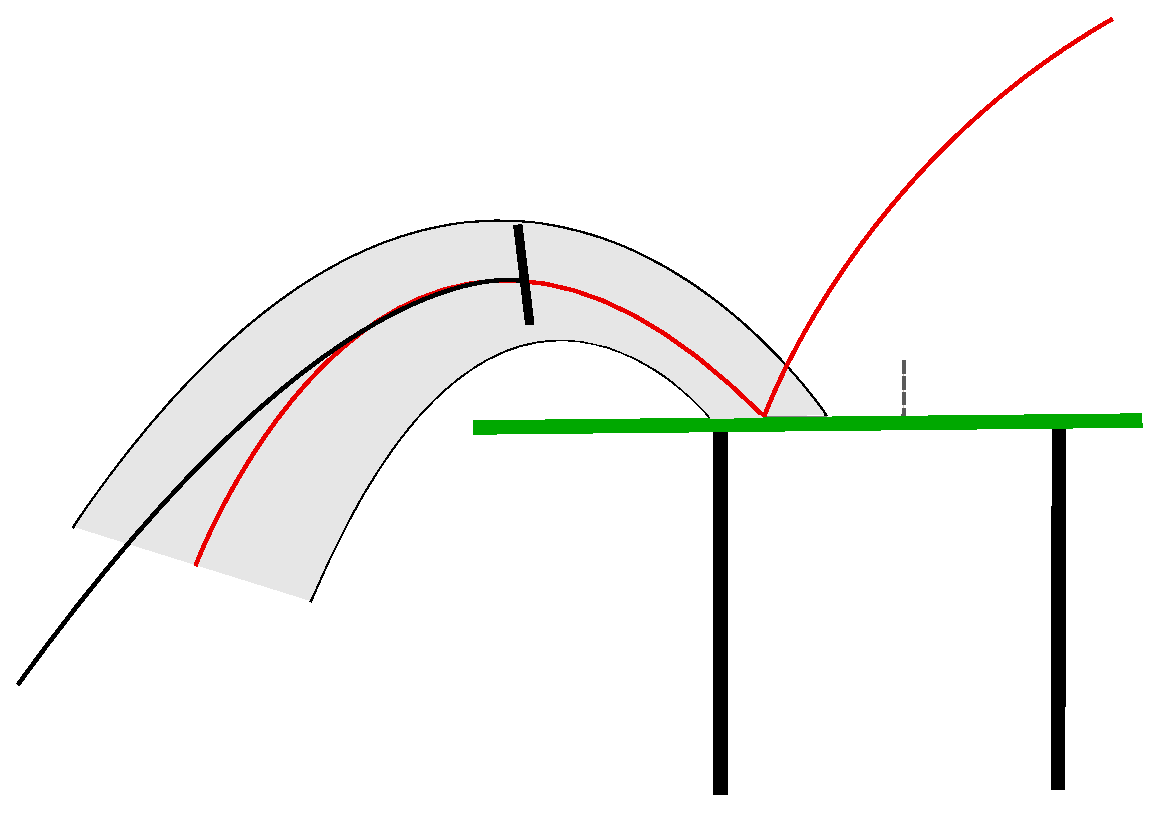
\includegraphics[scale=0.4]{drawing.eps}			
\caption{Illustrating the main idea behind this paper: from the ball's point of view, a racket trajectory in table tennis has a certain probability of hitting the ball and a significantly smaller probability of landing it (legally) on the opponents court. From the racket's point of view, the ball motion is a certain stochastic process and it should be intercepted such that the marginal probability distribution at hitting time is transformed at landing time to a desired marginal distribution. Racket trajectory and the mean of the ball trajectory are shown in black and red, respectively. }
\label{mainIdea}
\end{figure}

\section{RELATED WORK}\label{relatedWork}

% % % % Striking Movement Generation in Humans % % % % %
% speed-accuracy trade-off [Woodworth 1899, Fitts 1954]
% variability [Todorov and Jordan, 2002]
% goal-directed corrections [Elliott et al.]
% biomechanical redundancy [Bernstein, 1967]
% cost functions from optimal control [ Bryson and Ho, 1975; Hogan, 1984; Harris and Wolpert, 1998; Todorov and Jordan, 2002]
% motor program [Henry and Rogers, 1960; Keele, 19658; Schmidt, 1975; Schmidt and Wrisber, 2000, Schmidt, 2003]
% related: operational timing hypothesis [Tyldesley and Whiting, 1975]
% tau hypothesis to account for the time-to-contact: tau is specified as the relative inverse rate of dilation of the object image [Lee and Young, 1985; evidence for it: Bootsma and van Wieringen, 1988]
% stroke timing independent of ball speed [Hubbard and Seng, 1954] 
% error tolerance [Dagmar Sternad, Hermann Mueller, 2011]
% funnel-like control with fixed spatio-temporal bandwidth [Bootsma and Peper, 1992; Williams and Starkes, 2002]

% % % % Cost functions for movement generation % % % %
% cost of the movement includes - jerk, (metabolic) energy [Bryson and Ho, 1975]
% relationships found in reaching and pointing movements do not hold in striking sports [Bootsma and van Wieringen, 1990]
% energy optimality [Alexander, 1997; Kuo, 2005]
% Comfort of the posture, i.e. cost is induced by proximity to a fixed comfort posture in joint-space. 
% We believe that a new performance criterion in robotic table tennis is needed to explain the robust trajectory generation frequently observed in humans, and in order to compete with them. 

% robust movement generation
% robust algorithms that can compensate for low quality hardware and uncertainty in ball estimation

% hitting stage lasts approximately 80 ms in expert humans [only find a robust hitting trajectory]

% make sure to cite Marco Campi's scenario approach in robust control
% cite Stochastic Minimum Principle papers

\section{METHOD}\label{method}

In table tennis, one needs to determine when, where and how to intercept the incoming ball trajectory. So far, most of the algorithms for robotic table tennis \cite{Muelling13} calculate the intersection point of an estimated ball trajectory with a Virtual Hitting Plane (VHP) to determine the space and time coordinates of the hitting point. To estimate the trajectory of the ball, we require as data, a stream of estimates of ball position. We terminate the estimation process after a bounce event has been detected with high probability. 
% do we really need a fixed event such as bounce to terminate the estimation process?
%It is possible to eliminate this termination event altogether and vary the robot trajectory launch times based on ball estimates.

For safety reasons, VHP algorithms need to specify a minimum hitting time $T_{\textrm{min}}$ in addition to the coordinates of the hitting plane. When the ball is coming very fast towards the VHP, any calculated trajectory of duration below the minimum time will simply not be executed. This will prevent high accelerations and any risk of damage to the robot. However the determination of this minimum hitting time can be arbitrary, and the algorithms involving a VHP can lead to unnecessarily strict or restrictive strokes.
% impact time, ball position and velocity
% time to contact

After accounting for the net and any other environmental constraints such as walls, the stability region of table tennis reduces to the Cartesian coordinates of the table $\court$ as a rectangular region with a fixed vertical distance $z_{\court}$ from origin. Any algorithm that can return the ball to this fixed region can be said to be \emph{stable}.


\subsection{Learning Models From Data}

% air resistance scale factor C 
% $\ballFull = (\ball^{\mathrm{T}},\dot{\ball^{\mathrm{T}}})^{\mathrm{T}}$
We require three models for the trajectory generation process and acquire them (iteratively) from raw ball data. The ballistic \emph{flight model} $\ddot{\ball} = \ballDynamics(\dot{\ball})$ is a nonlinear model that describes the ball dynamics and generally involves air drag $\drag$ and gravity $\gravity$. The \emph{rebound model} $\dot{\ball}_{\mathrm{out}} = \bounce\dot{\ball}_{\mathrm{in}}$ is a discrete event with diagonal entries of $\bounce$ as coefficients $\epsilon = [\epsilon_{x}, \epsilon_{y}, -\epsilon_{z}]$. The coefficient of restitution $\epsilon_{z}$ accounts for the reflection of velocity in the vertical direction $z$ and $\epsilon_{x}, \epsilon_{y}$ are the coefficients of friction along the planar $x,y$ directions.
% incoming ball trajectory: as Gaussians indexed with time [e.g. Kalman filter should give us this information with prediction. Parameters/model of a Kalman filter could be fit using ball data (when fitting, innovation of the KF should be minimized as to consist mostly of white noise)]

% A probabilistic model describing the interaction model: outputs a probability distribution of outgoing ball states parameterized (or indexed) by t, e.g. b_t \approx N(\mu_b_out(t), \sigma_b_out(t))

% build a forward/inverse interaction model probabilistically
The last model to train from data is the \emph{ball-racket contact model} $\ \dot{\ball}_{\mathrm{out}} = \contact(\dot{\ball}_{\mathrm{in}},\dot{\racket},\orient)$. This model is significantly harder to train from the previous models, as it requires ball-racket interaction data and it is difficult to get reliable ball estimates around hitting time. We need to instead rely on smoothing using the trained flight model and the samples before and after hitting. In previous works, the outgoing velocity of the ball is calculated using a \emph{mirror law}: $o_{\parallel} - v = \epsilon_{R} (-i_{\parallel} + v)$ with $v$ the speed of the racket along its normal and $\epsilon_{R}$ the coefficient of restitution on the racket. $o_{\parallel}$ and $i_{\parallel}$ are the outgoing and incoming ball velocities along the racket, respectively. This model assumes an elastic momentum exchange and it is quite inaccurate, especially at high ball velocities.
% is this true? is the parallel o and i definitions correct?

The accuracy of these models all depend on each other and for this reason, we train the parameters of these models with the Expectation-Maximization (EM) algorithm. Effects of angular velocity, or in other words spin, are not accounted for in these models. During test time when running these trained models online, an Extended Kalman Filter (EKF) or any regression method to estimate initial ball position and velocity can use these models to perform prediction and update steps.

\subsection{Predicting with Probabilistic Modeling}

% density or distribution
Using an EKF for our nonlinear model $\ballDynamics$ generates at each time instant $t$ a probability distribution $p_t(x,y,z|t)$ of incoming ball states parameterized by time, e.g. $\ball_t \sim \mathcal{N}(\vec{\mu}_{\textrm{in}}(t),\vec{\Sigma}_{\textrm{in}}(t))$. 

% % % EXT. KALMAN FILTER EQUATIONS HERE % % %

Formally this is a stochastic process, and for the Kalman Filter with a noisy process model, a Brownian motion. However we set the process covariance to zero during prediction, as the sample paths of the exponential kernel used in the Kalman Filter framework are very rough, i.e. almost surely not differentiable.

% Interaction probabilities (ball touching the racket)
Prediction continues after a possible interaction with the racket trajectory. If the ball touches the racket, i.e. if the surface of the ball is located inside the radius $\racketRadius = 8$ cm of the racket plane, ball incoming velocities will be transformed according to the trained contact model. Otherwise the ball with continue its previous projectile-like motion. Prediction is stopped when the ball hits the table plane with negative velocity in the $z$ direction.

\subsection{Optimal Control for Trajectory Generation}

From a set point of view, for every point on the predicted ball trajectory, there is a range of admissible outgoing ball velocities that the racket can impart. This set is constricted by the geometry of the table and the demands of the game: the ball has to avoid the net and the walls and should land on the opponents court. Probabilistically speaking, the landing point could be any distribution with compact support over the table, e.g. a uniform distribution $x_{\textrm{land}}, y_{\textrm{land}} \sim \mathcal{U}(\court) = \mathcal{U}(x_{a},x_{b})\mathcal{U}(y_{a},y_{b})$ or a truncated normal distribution. The limiting values $x_{a},x_{b},y_{a},y_{b}$ are obtained from the rectangular geometry of the opponent's court.
%

Our optimization criterion of choice is to find the racket trajectory that minimizes the Kullback-Leibler (KL) divergence $\textrm{KL}(p\|q) = \int_{\court}p(x,y)\log(\frac{p(x,y)}{q(x,y)})\textrm{d}x\textrm{d}y$ of $p(x,y|z_{\court},\dot{z} < 0) = \int_{\hitTime = 0}^{\infty} p_{\hitTime}(x,y|z_{\court},\dot{z} < 0,\hitTime)\hitDist \textrm{d}\hitTime$ with a desired distribution imposed by the robotic player. $p(x,y|z_{\court},\dot{z} < 0)$ is the marginal distribution over time of the ball process $p_t(\cdot)$. Other more agnostic optimization criteria could also be formulated to minimize the racket trajectory sensitivity to perturbations in the ball trajectory. However these would not take advantage of the uncertainty quantification of the ball trajectory, in our case supplied by EKF.

% what about maximizing the probability of landing, regardless of any specified distribution?
% is this true?
Any specified distribution $q(\cdot)$ of compact support $\court$ will indirectly maximize the probability of landing on the table, $\prob(\textrm{land}) = \int_{0}^{\infty}\landDist\textrm{d}\landTime$. Here $\landTime$ is a \emph{hitting time} random variable of the set $\court$. In addition, for maximal unpredictability, the robot player can choose the uniform distribution over the table as a desired distribution. In this case the optimization reduces to maximizing the entropy of the landing distribution on the table. 

For safety and efficiency, we would prefer trajectories with minimal acceleration or jerk, the derivative of acceleration. Combining the minimal acceleration criterion with the KL-divergence we get
%
\begin{align}
\min \int\limits_{0}^{T}\ddot{\joint}(t) + \textrm{KL}(p(x,y|z_{\court},\dot{z}<0)|\mathcal{U}(\court)),
\label{costFnc1}
\end{align}
%
where the marginal distribution $p(x,y|z_{\court},\dot{z}<0)$ of the ball process can be written as
%
% should we give also the probability of landing here?
\begin{align}
p(x,y|z_{\court},\dot{z}<0) &= \int_{\landTime = 0}^{\infty} p_{\landTime}(x,y|z_{\court},\dot{z}<0,\landTime)\hitDist \textrm{d}\landTime \label{marginalDistr1}, \\
p_{\landTime}(x,y|z_{\court},\dot{z}<0,\landTime) &= \frac{ \int_{\dot{z}=-\infty}^{0}\int_{\dot{x},\dot{y}}p_{\landTime}(x,y,z_{\court},\dot{x},\dot{y},\dot{z}|\landTime)}{p(z_{\court},\dot{z}<0)}.
\label{marginalDistr2}
\end{align}
%
The marginal distribution over $x,y$ velocities appearing in the numerator of \eqref{marginalDistr2} is
\begin{align}
& p_{\landTime}(x,y,z,\dot{z}|\landTime) = \int_{\hitTime = 0}^{T} \int_{\dot{x},\dot{y}}  p_{\landTime}(x,y,z,\dot{x},\dot{y},\dot{z}|\ball_{\textrm{out}},\dot{\ball}_{\textrm{out}},\landTime) \times \\
& p(\dot{\ball}_{\textrm{out}}|\dot{\ball}_{\textrm{in}},\dot{\racket}(\hitTime),\orient(\hitTime),\hitTime)p(\ball_{\textrm{out}}|\ball_{\textrm{in}},\racket(\hitTime),\orient(\hitTime),\hitTime)\hitDist\textrm{d}\hitTime.
\label{fullDistr}
\end{align}
%
where $\hitTime$ is the hitting time random variable corresponding to the time of ball-racket contact, $\prob(\textrm{hit}) = \int_{0}^{T}\hitDist\textrm{d}\hitTime$. In \eqref{fullDistr} the probability densities are obtained using the trained models, i.e. the flight model and the ball-racket contact model. 

By formulating \eqref{costFnc1} in joint space, we find the joint trajectory $\joint(t)$ that provides a suitable trade-off between minimum joint accelerations $\ddot{\joint}(t)$ and maximum probability of landing $\prob(\textrm{land})$. Using direct kinematics we can obtain the desired racket trajectory and orientations, i.e. $[\racket(t),\orient(t)] = \kin(\joint(t))$.




% Output
% 
% The mapping r_t \approx N(\mu_racket_center(t),\sigma_racket_center(t))) as racket reference trajectory that maximizes the probability of landing on the opponents court, or minimizing KL-divergence between outgoing ball states distribution and admissable/desired velocities [e.g. uniform distribution of velocities]

% Control: imposing transversality conditions when ball is on a curve p_b(t) or a set with some measure p_b [constant hamiltonian on this set?] we get a probability distribution of admissable end effector configurations
%
%
% Probability of interaction occurring: b(t) for the ball must lie in r(t) + \gamma o_\parallel(t), where r(t) is the racket centre trajectory, \gamma is less than the radius of the racket, and o_\parallel(t) is any direction perpendicular to the normal (i.e. orientation) of the racket.
%

% Refer to article for the simplest case when diving two Gaussians with nonzero mean.
We do not know of any way to compute the ball landing distribution in closed form, as a function of racket positions and orientations. However, the outgoing ball trajectory is an integral over the previous incoming ball distribution using the ball-racket contact model. Any sampling based approach (e.g. rejection sampling) may be used to simulate then the outgoing ball trajectory and approximate the resulting landing distribution. 


\section{ALGORITHM}\label{alg}

\section{EXPERIMENTS}\label{results}

% % % CHANGE THE WRITING HERE !!! OTHERWISE ITS THE SAME AS PREVIOUS ARTICLE

% % % % Table Tennis Setup % % % %
For the robotic table tennis task we are using a seven degree of freedom (DoF) torque-controlled custom made Barrett WAM arm capable of high speeds and accelerations. A standard size racket (16 cm diameter) is mounted on the end-effector of the arm as can be seen in Figure~\ref{robot}. A vision system consisting of four cameras hanging from the ceiling around each corner of the table is used for tracking the ball \cite{Lampert12}. The orange ball is tracked visually with a sampling rate of 60 Hz and filtered with an EKF that accounts for some of the bouncing behavior of the ball and air drag effects. The table and the tennis balls are in accordance with the International Table Tennis Federation (ITTF) rules.
%
A ball launcher (see Figure~\ref{robot}) is available to throw balls accurately to a fixed position in Cartesian space to the forehand of the robot. The incoming ball arrives with low-variability in desired positions and higher-variability in ball velocities. The whole area to be covered amounts to about 1 m$^2$ circular region surrounding the initial forehand posture of the robot. This allows us to avoid the singularities of the robot. Any ball that appears outside of this circular \emph{feasible} region will not be hit.
%
After the visual system predicts a ball trajectory that coincides with the feasible region in Cartesian space, the motion planning system has to come up with a trajectory that specifies how, where and when to intercept the incoming ball. 
%Desired Cartesian position, velocity and orientations of the racket translate in joint space to a specification of 14 parameters: 7 joint angles and 7 joint velocities of the robot arm. Along with the desired hitting time (or the time until impact), these 15 parameters are used to train 7 joint space trajectories that correspond to the desired reference trajectory in Cartesian space.
%
In runtime, in order to generate feasible reference trajectories that account for the variations in incoming ball position and velocities, we run the robust trajectory generation framework $\alg$. We start these joint reference trajectories from the initial posture of the robot provided by the sensors.
% From Katharina's paper:
%the position, velocity and orientation of the racket can be computed analytically based on the state of the system and the target on the opponents court.
%These task space parameters can also be converted into joint space parameters using inverse kinematics

Due to the limitations of our setup, our robot is fixed to the ceiling. Hence we expect that the balls that hit the frontal areas of the robots table will not be hit. The table can be brought closer to the robot to overcome this limitation: however then the trajectory generation problem will be subsequently harder, and the hard constraint of hitting the table becomes more problematic to avoid.

% vision system operates in a semi-structured and human-inhabited environment
% Finite State Automaton: four stages: awaiting stage, preparation, hitting and finishing stage

\section{CONCLUSION}\label{end}

% stochastic optimal control
We see the probabilistic extensions of Pontryagin's minimum principle as a very fruitful direction for robotics in general in the upcoming years, as robots start taking decisions in complex, demanding tasks. The robot trajectories to be generated can also taken to be probabilistic, leading to an optimization framework that considers the interaction between two probability distributions. We consider the probabilistic movement primitives~\cite{Paraschos13} to be a step in the right direction.

% reinforcement learning to modify trajectories

The cost functional to be minimized considers the accelerations as the quantity to be minimized. It assumes that the feedback linearization of the robot is perfect, that is the inverse dynamics model for the robot is exact. Whenever the cancellation is imperfect due to inaccurate robot control, execution error will prevent the robot from achieving the desired trajectories. Execution errors are not taken into consideration within this framework. 

A natural reward signal to use for reinforcement learning is to look at the set-distance of the landing point from the opponents court. This reward can be used to modify the generated trajectories and learn to compensate for the execution errors. Another promising approach is Iterative Learning Control (ILC), see for example \cite{Bristow06}, \cite{Longman2000}, \cite{Koc15}. ILC is a more efficient learning approach that generally makes more assumptions. Generalizing ILC to different trajectories generated by $\alg$, we hope to increase the performance of our robot further. 

\bibliographystyle{plain}
%\bibliographystyle{./IEEEtran}
%\bibliography{./IEEEabrv,./iros2015Ref}
\bibliography{./ttRef}

\end{document}
